\documentclass{article}
\usepackage[final,nonatbib]{aaj2026}
% Fallbacks for a local compile only: \providecommand does nothing where the
% Overleaf project already defines these commands.
\providecommand{\affilmark}[1]{\textsuperscript{#1}}
\providecommand{\affiliations}[1]{}
\providecommand{\correspondence}[1]{}

\usepackage[utf8]{inputenc}
\usepackage[T1]{fontenc}
\usepackage{float}
\usepackage{placeins}
\usepackage{enumitem}

\usepackage[
  backend=biber,
  style=ieee,
  sorting=none
]{biblatex}
\addbibresource{refs.bib}
\addbibresource{refs_methods_additions_20261003.bib}

\usepackage{url}
\usepackage{booktabs}
\usepackage{amsfonts}
\usepackage{amsmath}
\usepackage{amssymb}
\usepackage{nicefrac}
\usepackage{microtype}
\usepackage{xcolor}
\usepackage{multirow}
\usepackage{tabularx}
\usepackage{array}
\usepackage{graphicx}
\usepackage{tikz}
\usetikzlibrary{positioning,arrows.meta,fit,calc}
\usepackage[hidelinks,breaklinks=true]{hyperref}

\graphicspath{{figures/}}
% Values that come from the measurement-noise batch still running
% (results/batches/noise_20260927_134251). Replace every \pending{} once
% aggregate_noise_simulation has written summary/.
\newcommand{\pending}[1]{\textcolor{red}{[#1]}}

\title{Patient-Specific Lumped-Parameter Model for Quantifying Shunt Flow and Predicting Post-Closure Hemodynamics in Pediatric Ventricular Septal Defect}

\author{%
  Puspita Anggraini Katili\affilmark{1,*} \and
  Muhammad H.~A.~Subagyo\affilmark{1} \and
  Aisyah M.~Dzakiyah\affilmark{1} \and
  Sylvi Febriana Rachmawati Irnadiastputri\affilmark{1} \and
  Winda Azwani\affilmark{2}%
}
\affiliations{%
  \affilmark{1}Biomedical Engineering Program, Department of Electrical Engineering,\\
  Universitas Indonesia\\[2pt]
  \affilmark{2} RSAB Harapan Kita, Jakarta, Indonesia\\[4pt]
}

\correspondence {puspita.katili@ui.ac.id}

\begin{document}
\maketitle

\begin{abstract}
Ventricular septal defect (VSD) is one of the most common congenital heart defect which usually be closed using a closure procedure based on transcatheter. Although closure is usually successful, individual heart characteristics and chamber remodelling can cause a problem in pre-surgery planning, which can make the results become unpredictable. Computer modelling based on Lumped Parameter Model (LPM) has been used in wide range of congenital heart defects problem. However, relatively small amount of studies have build it directly for VSD patients, let alone on a patient-specifics model which persists on its pre and post closure surgery prediction. We scaled a closed-loop zero-dimensional LPM with an orifice model of the defect by body weight to a 3.2-year-old, 13.4-kg girl with a restrictive perimembranous VSD ($Q_p/Q_s = 1.19$), and selected the parameters to calibrate by variance-based global sensitivity analysis. Seven of 14 candidate parameters were retained, led by systemic resistance, the defect discharge coefficient and right-ventricular passive elastance. Multi-start calibration to nine pre-closure catheterization targets reduced the root-mean-square relative error from 0.274 to 0.105. The calibrated parameters were then applied unchanged with the defect closed to predict the post-closure state. The seven post-closure catheter pressures were predicted with a root-mean-square error of 6.9~mmHg, against 5.2~mmHg for the same pressures fitted before closure, with relative errors of $+1.2\%$ for systolic and $-6.4\%$ for mean arterial pressure. The largest errors were in systolic pulmonary arterial pressure ($+40.7\%$), carried over from calibration, and right-ventricular end-diastolic volume ($+42.1\%$), which no pre-closure measurement constrains. \pending{Noise-simulation sentence once the batch finishes.} In this child, the pre-closure calibration predicted post-closure pressures but not chamber volumes; predicting volumes would require a pre-closure volume measurement.
\end{abstract}

\noindent\textbf{Keywords:} Ventricular septal defect, lumped-parameter model, patient-specific modeling, global sensitivity analysis, parameter identifiability, congenital heart disease

% =====================================================================
\section{Introduction}

Congenital heart disease (CHD) is one of the most common birth defects, with a global prevalence estimated to be 9.41 per 1,000 live births during 2010--2017, 10\% higher than the previous 15 years~\cite{Liu2019}. Ventricular septal defect (VSD) is one of the most common types of CHD with an incidence of 3.07 per 1,000 live births and accounting for 35.6\% of all CHD cases worldwide~\cite{Liu2019,vanderLinde2011}. In Indonesia alone, 43,200 infants are born each year with CHD and early detection is limited outside large population centers~\cite{Marwali2021}. VSD creates an abnormal channel between the ventricles, which causes the blood to be shunted across the chambers. The shunt depends on the defect size, the interventricular pressure gradient, and the ratio of pulmonary to systemic vascular resistance~\cite{Sommer2008,Rao2024}. A left-to-right shunt increases the pulmonary blood flow and left-heart volume loading when it becomes hemodynamically significant, which, if left untreated, can lead to heart failure and pulmonary vascular remodeling~\cite{Sommer2008,Arvanitaki2022}. While many small defects close spontaneously during early childhood, larger defects and certain anatomical subtypes do not, leaving a group of children who require closure~\cite{Zhang2015Spontaneous,Li2019Spontaneous}.

Transcatheter closure is often preferred because it avoids cardiopulmonary bypass in anatomically suitable cases~\cite{Turner2022,Ali_Hassan_2019}. However, the procedure itself does not guarantee a successful hemodynamic course, as 36.4\% of children still have residual shunting immediately after transcatheter closure, and 9.8\% still have residual shunting at follow-up~\cite{Vuran2026}. Another study reported 3.1\% of children requiring unplanned surgery after device closure due to new or worsening aortic regurgitation~\cite{Yang2021Surgery}. Residual shunt and worsening aortic regurgitation are associated with a larger defect and younger age~\cite{Chin2024}, while low body weight is associated with adverse events after surgical closure~\cite{Abdelrehim2022}. The hemodynamic state after closure therefore varies between children and is not known before the procedure.

Echocardiography characterizes the pre-closure state but is operator-dependent and prone to diagnostic error in young children~\cite{Benavidez2008}. At the same time, cardiac catheterization, which is considered the gold standard, captures only a single physiological state~\cite{Feltes2011}. Neither modality predicts how a patient's pressures, flows and chamber volumes will change once the shunt is removed. A quantitative and predictive patient-specific model would therefore be useful in predicting the hemodynamic outcome of closure before the procedure. Patient-specific computational models combine clinical measurements with mathematical modeling to reconstruct a patient's hemodynamics and simulate states that have not yet occurred~\cite{Taylor2009}. In cardiology, such models have been used to plan surgical intervention or evaluate the disease progression~\cite{Marsden2015,Pennati2013}. Such models are often built with three-dimensional computational fluid dynamics, but their computational cost limits repeated use~\cite{Pennati2013}. Zero-dimensional lumped-parameter models (LPMs) offer an alternative at a fraction of the cost~\cite{Shi2011}.

LPMs have been applied across congenital and pediatric conditions. Shimizu et al.\ developed LPMs across several CHD configurations and reproduced the hemodynamics of each configuration~\cite{Shimizu2018}, while Schiavazzi et al.\ estimated the parameters of a closed-loop circulation under measurement uncertainty~\cite{Schiavazzi2017}. Horio et al.\ used an LPM to estimate pressure and flow in Fontan circulations~\cite{Horio2024}. Bozkurt developed a model that simulates cardiac function and chamber dimensions in adults and children~\cite{Bozkurt2019} and optimized its parameters to reproduce measurements in three children with dilated cardiomyopathy~\cite{Bozkurt2022}. For specific VSD models, Lee and Jung coupled a three-dimensional heart to lumped circulation to simulate VSD flow~\cite{Lee2015}, while Ferrero et al.\ used a 0D framework to interpret the catheterization data from patients with intracardiac shunts but did not predict a post-intervention state~\cite{Ferrero2026Shunts}. Most recently, Colebank et al.\ combined an eight-compartment LPM with age-dependent parameters to simulate small, medium, and large VSD from birth to two years of age, without calibration to individual children~\cite{Colebank2026}.

Despite this progress, computational studies of VSD remain scarce~\cite{Colebank2026}, and to our knowledge, no VSD model has been calibrated to an individual child and then tested against the same child's post-closure measurements. Two problems arise when these models are applied to a child. First, the adult reference parameters cannot be directly used on a small child. The model must be scaled by body weight or body surface area to reproduce the age-related changes from infancy to adolescence~\cite{zhang2019multiscale,Lundquist2025}. Second, patient-specific models usually contain more parameters than the available clinical measurements can determine, which constrains the model's accuracy~\cite{Schiavazzi2017}. Global sensitivity analysis can address this by identifying the most influential parameters, allowing less influential ones to be fixed and reducing the number to be estimated~\cite{Saltelli2010,vanOsta2020}. A test against post-closure measurements shows which post-closure quantities a pre-closure record can predict, and that answer depends on which parameters the pre-closure data determine and on how measurement error propagates to the prediction. The aim of this study is to develop a patient-specific LPM of pediatric VSD, which is calibrated to pre-closure clinical data and used to predict the post-closure circulation of the same patient. Specifically, we (i) scale the model to the child by body weight; (ii) select the calibration parameters by variance-based global sensitivity analysis and estimate them by multi-start optimization; (iii) predict the post-closure state without refitting and compare it with catheterization and echocardiography measurements acquired from clinical records; and (iv) quantify how pre-closure measurement uncertainty propagates to the calibrated parameters and the prediction. To our knowledge, this is the first study that calibrates a pediatric VSD model to a child's pre-closure measurements and then tests its prediction against the same child's post-closure measurements.

% =====================================================================
\section{Materials and Methods}
\label{sec:methods}
Figure~\ref{fig:workflow} summarizes the workflow: the clinical record, pediatric scaling and clinical seeding, the sensitivity screen, calibration, the post-closure prediction and the measurement-noise simulation.

\subsection{Patient}
\label{sec:study_population}
The patient was enrolled in a prospective modeling study of children scheduled for transcatheter VSD closure at the National Center for Women and Children's Health, RSAB Harapan Kita, Jakarta, Indonesia (December 2025 to June 2026). Children older than three months with an echocardiographically confirmed VSD larger than 2~mm were eligible; children with an additional severe cardiovascular abnormality or previous cardiac intervention were excluded. The first child enrolled with a complete catheterization and echocardiographic record both before and after closure is the subject of this study; to keep the data de-identified, she is referred to as P1 (patient 1 of the study). P1 was a 3-year-old girl (age 3.17~years, weight 13.4~kg, height 95~cm) with a perimembranous outlet VSD measuring 5.4~mm on the left-ventricular side and 3.7~mm on the right-ventricular side. The study was approved by the Institutional Review Board of RSAB Harapan Kita (DP.04.03/D.XXII/4749/2025); written informed consent was obtained from the patient's legal guardian.

\subsection{Clinical data}
\label{sec:data}
Clinical data were obtained from the catheterization protocol forms and the medical record (Table~\ref{tab:patient_data}). The defect diameter was measured on echocardiography at both ventricular sides; the right-ventricular side, which is the narrower, restrictive orifice, was used as the model input, taken as the mean of the recorded range of 3.63--3.70~mm ($D_{\mathrm{VSD}} = 3.665$~mm). Heart rate was recorded separately for each state (119~bpm before and 108~bpm after closure) and used as a model input in that state. Where the form records three consecutive readings, the median was used.

Pressures were recorded with a hydrophilic angiographic catheter (APT Medical, Shenzhen, China). Mean arterial pressure was computed from the right femoral artery (RFA) catheter readings with the formula of the catheterization protocol, $\overline{P} = (P_{\mathrm{sys}} + 2P_{\mathrm{dia}})/3$; the mean arterial pressure entered on the form is computed from the cuff readings and was not used. Pulmonary flow $Q_p = 4.087$~L/min and $Q_p/Q_s = 1.194$ were measured by the Fick method during catheterization, with blood oxygen saturations measured on an AVOXimeter 1000E whole-blood co-oximeter (Accriva Diagnostics, San Diego, CA, USA). Systemic flow and shunt flow were derived from them as $Q_s = Q_p/(Q_p/Q_s) = 3.423$~L/min and $Q_{\mathrm{shunt}} = Q_p - Q_s = 0.664$~L/min. Systemic vascular resistance was derived as $(\overline{P} - P_{\mathrm{RA}})/Q_s$; pulmonary vascular resistance could not be derived because left atrial pressure was not measured.

The ventricular volumes after closure were measured by echocardiography with the device deployed and occluding the defect, before its release: left-ventricular volumes by the biplane method and right-ventricular volumes by three-dimensional echocardiography. Invasive pressures were recorded by catheter 9--26~min after device release, in the same session and under the same anaesthesia as the pre-closure measurements. The medical record gives a second set of left-ventricular volumes (LVEDV/LVESV 36.13/13.80~mL), which is the primary comparison; the protocol-form values (32.0/23.6~mL) are evaluated as an alternative.

\begin{table}[!htbp]
\centering\small
\setlength{\tabcolsep}{3.5pt}
\caption{Clinical record of P1 used in this study. Values marked with an asterisk are the targets of the pre-closure calibration; all other values are compared with the model only. No post-closure value was used in calibration.}
\label{tab:patient_data}
\resizebox{\linewidth}{!}{\begin{tabular}{llrr}
\toprule
\textbf{Variable} & \textbf{Method} & \textbf{Pre-closure} & \textbf{Post-closure} \\
\midrule
\multicolumn{4}{l}{\emph{Model inputs}} \\
Age (yr) & medical record & 3.17 & 3.17 \\
Weight (kg) & measured & 13.4 & 13.4 \\
Heart rate (bpm) & ECG monitor & 119 & 108 \\
VSD diameter, RV side (mm) & echocardiography & 3.665 & -- \\
\midrule
\multicolumn{4}{l}{\emph{Pressures (mmHg)}} \\
Systolic / diastolic pressure, RFA & catheter & 100$^{*}$ / 57$^{*}$ & 89 / 68 \\
Mean arterial pressure, RFA & $(P_{\mathrm{sys}} + 2P_{\mathrm{dia}})/3$ & 71.33$^{*}$ & 75.00 \\
Systolic / diastolic pressure, DAo & catheter & 91 / 57 & 104 / 72 \\
Systolic / diastolic pressure, cuff & oscillometric & 119 / 83 & 87 / 55 \\
PA pressure, sys / dia / mean & catheter & 20$^{*}$ / 10$^{*}$ / 15$^{*}$ & 17 / 9 / 13 \\
RA mean pressure & catheter & 5$^{*}$ & 5 \\
LV / RV systolic pressure & catheter & 94 / 25 & -- \\
LV--RV peak systolic gradient & LV $-$ RV & 69 & -- \\
\midrule
\multicolumn{4}{l}{\emph{Flows and resistance}} \\
Pulmonary flow $Q_p$ (L/min) & Fick & 4.087 & -- \\
$Q_p/Q_s$ (--) & Fick / echocardiography$^{\mathrm{a}}$ & 1.194$^{*}$ & 0.90 \\
Systemic flow $Q_s$ (L/min) & $Q_p/(Q_p/Q_s)$ / echocardiography$^{\mathrm{a}}$ & 3.423$^{*}$ & 2.54 \\
Shunt flow (L/min) & $Q_p - Q_s$ & 0.664$^{*}$ & -- \\
SVR (WU) & $(\overline{P} - P_{\mathrm{RA}})/Q_s$ & 19.38 & 27.56 \\
\midrule
\multicolumn{4}{l}{\emph{Ventricular volumes and function}} \\
LVEDV / LVESV (mL) & echocardiography, biplane$^{\mathrm{a}}$ & -- & 36.13 / 13.80$^{\mathrm{b}}$ \\
RVEDV / RVESV (mL) & echocardiography, 3D & -- & 30.5 / 12.0 \\
LVEF / RVEF (--) & from volumes & -- & 0.618 / 0.607 \\
\bottomrule
\end{tabular}}
\par\vspace{2pt}
\begin{minipage}{0.97\linewidth}
\raggedright\footnotesize
\emph{Abbreviations:} DAo, descending aorta; EDV/ESV, end-diastolic/end-systolic volume; EF, ejection fraction; LV/RV, left/right ventricle; PA, pulmonary artery; RA, right atrium; RFA, right femoral artery; SVR, systemic vascular resistance.\\
\emph{Note:} Values are from the catheterization protocol forms except where marked. $^{\mathrm{a}}$Post-closure value from the medical record. $^{\mathrm{b}}$The protocol form gives 32.0 / 23.6~mL; this alternative record is evaluated in Section~\ref{sec:results_post}.
\end{minipage}
\end{table}

% ---------------------------------------------------------------------
\begin{figure}[!htbp]
\centering
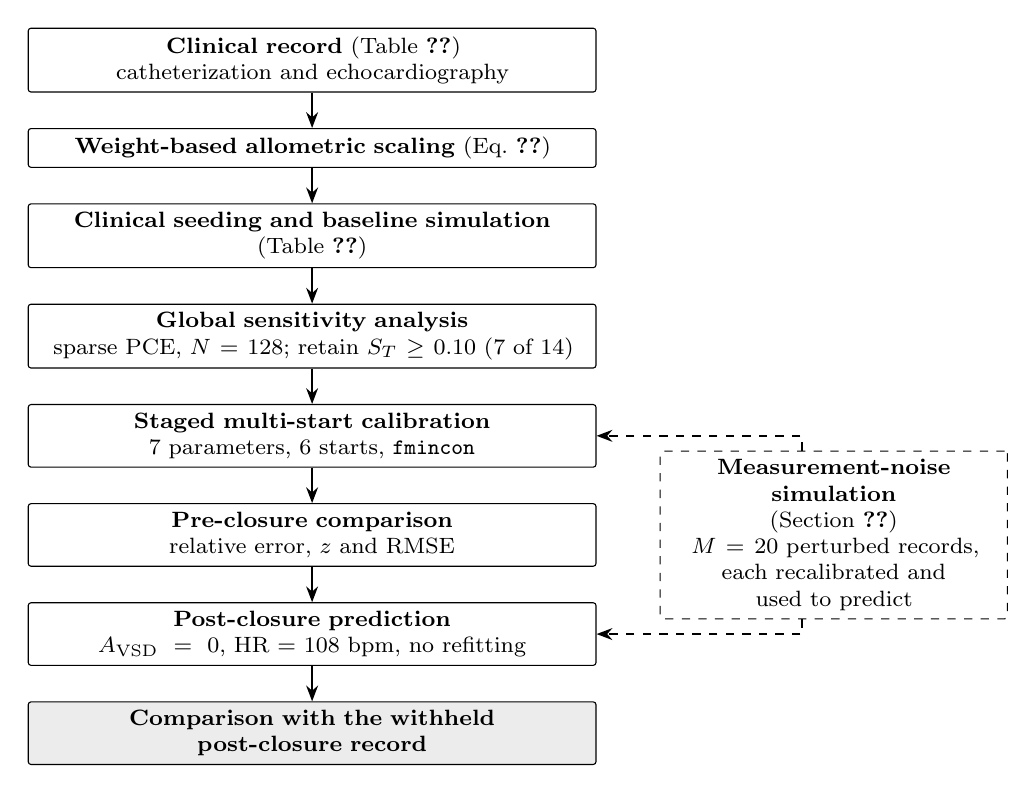
\begin{tikzpicture}[
  node distance=4.5mm,
  every node/.append style={execute at begin node={\hyphenpenalty=10000 \exhyphenpenalty=10000}},
  box/.style={draw, rounded corners=1pt, align=center, font=\footnotesize, text width=7.0cm, inner sep=3pt, fill=white},
  sbox/.style={draw, dashed, rounded corners=1pt, align=center, font=\footnotesize, text width=4.2cm, inner sep=3pt},
  arr/.style={-{Stealth[length=2mm]}, thick}]
\node[box] (clin) {\textbf{Clinical record} (Table~\ref{tab:patient_data})\\ catheterization and echocardiography};
\node[box, below=of clin] (scale) {\textbf{Weight-based allometric scaling} (Eq.~\ref{eq:scaling})};
\node[box, below=of scale] (seed) {\textbf{Clinical seeding and baseline simulation}\\ (Table~\ref{tab:seeding})};
\node[box, below=of seed] (gsa) {\textbf{Global sensitivity analysis}\\ sparse PCE, $N=128$; retain $S_T \ge 0.10$ (7 of 14)};
\node[box, below=of gsa] (cal) {\textbf{Staged multi-start calibration}\\ 7 parameters, 6 starts, \texttt{fmincon}};
\node[box, below=of cal] (eval) {\textbf{Pre-closure comparison}\\ relative error, $z$ and RMSE};
\node[box, below=of eval] (pred) {\textbf{Post-closure prediction}\\ $A_{\mathrm{VSD}} = 0$, HR = 108 bpm, no refitting};
\node[box, below=of pred, fill=gray!15] (cmp) {\textbf{Comparison with the withheld}\\ \textbf{post-closure record}};
\foreach \a/\b in {clin/scale, scale/seed, seed/gsa, gsa/cal, cal/eval, eval/pred, pred/cmp} \draw[arr] (\a) -- (\b);
\node[sbox, right=8mm of eval] (noise) {\textbf{Measurement-noise simulation}\\ (Section~\ref{sec:noise_methods})\\ $M=20$ perturbed records,\\ each recalibrated and\\ used to predict};
\draw[arr, dashed] ([xshift=-4mm]noise.north) |- (cal.east);
\draw[arr, dashed] ([xshift=-4mm]noise.south) |- (pred.east);
\end{tikzpicture}
\caption{Patient-specific modeling workflow. The clinical record scales and seeds the model, the sensitivity screen selects the seven fitted parameters, staged multi-start optimization calibrates the pre-closure state, and the calibrated parameters are applied unchanged with the defect closed to predict the withheld post-closure state. The measurement-noise simulation repeats calibration and prediction on perturbed records. PCE, polynomial chaos expansion; $S_T$, total-order Sobol' index; HR, heart rate.}
\label{fig:workflow}
\end{figure}

\FloatBarrier
\subsection{Mathematical model}
\label{sec:model}

\subsubsection{Structure}
The circulation is the closed-loop lumped-parameter model of Regazzoni et al.~\cite{Regazzoni2022}, in the version of Tonini et al.\ with oxygenated and non-oxygenated pulmonary capillary branches~\cite{Tonini2024,Tonini2025}, extended with an interventricular shunt by Valenti and Ferrero et al.~\cite{Valenti2023,Ferrero2026Shunts} (Figure~\ref{fig:schematic}). It contains four time-varying elastance chambers, a systemic circuit with arterial, capillary and venous compartments, a pulmonary circuit with an arterial compartment, two parallel capillary branches and a venous compartment, four valves and the shunt. Table~\ref{tab:components} lists the source of each component and what we changed. The model has 14 state variables,
\begin{equation}
\begin{split}\mathbf{X} = \big[ & V_{\mathrm{RA}}, V_{\mathrm{RV}}, V_{\mathrm{LA}}, V_{\mathrm{LV}}, V_{\mathrm{SAR}}, Q_{\mathrm{SAR}}, V_{\mathrm{SC}}, \\
  & V_{\mathrm{SVEN}}, Q_{\mathrm{SVEN}}, V_{\mathrm{PAR}}, Q_{\mathrm{PAR}}, P_{\mathrm{PC}}, V_{\mathrm{PVEN}}, Q_{\mathrm{PVEN}} \big]^{\top},\end{split}
\label{eq:state}
\end{equation}
with volumes $V$ (mL), flows $Q$ (mL/s) and the pulmonary capillary pressure $P_{\mathrm{PC}}$ (mmHg). The chamber volumes obey
\begin{equation}
\begin{aligned}
\dot{V}_{\mathrm{RA}} &= Q_{\mathrm{SVEN}} - Q_{\mathrm{TV}}, &
\dot{V}_{\mathrm{RV}} &= Q_{\mathrm{TV}} + Q_{\mathrm{VSD}} - Q_{\mathrm{PV}}, \\
\dot{V}_{\mathrm{LA}} &= Q_{\mathrm{PVEN}} - Q_{\mathrm{MV}}, &
\dot{V}_{\mathrm{LV}} &= Q_{\mathrm{MV}} - Q_{\mathrm{AV}} - Q_{\mathrm{VSD}},
\end{aligned}
\label{eq:chambers}
\end{equation}
where $Q_{\mathrm{TV}}$, $Q_{\mathrm{PV}}$, $Q_{\mathrm{MV}}$ and $Q_{\mathrm{AV}}$ are the flows through the tricuspid, pulmonary, mitral and aortic valves and $Q_{\mathrm{VSD}}$ is the shunt flow, positive from left to right. The vascular equations are given in Appendix~\ref{app:circuit} and the nominal adult values in Appendix~\ref{app:nominal_parameters}. The nominal values were obtained by manual tuning, starting from the adult values of Valenti~\cite{Valenti2023}, Zhang et al.~\cite{zhang2019multiscale} and Bozkurt~\cite{Bozkurt2019}, until the weight-scaled model of a healthy 3-year-old (14~kg, 98~cm, the WHO median for age~\cite{WHOgrowth}) matched pediatric reference ranges for heart rate~\cite{Joyce2025}, systemic blood pressure~\cite{Flynn2017} and pulmonary arterial and right atrial pressure~\cite{MalakanRad2024}. Supplementary Section~S6 lists every nominal value beside its three sources and every output of the healthy-child model beside its reference range. The external pressure on the chambers is zero, the two ventricles are not mechanically coupled through the septum, and valve regurgitation is not modelled.

\begin{table}[!htbp]
\centering\small
\caption{Model components, their source and the changes made in this work.}
\label{tab:components}
\resizebox{\linewidth}{!}{\begin{tabular}{lll}
\toprule
\textbf{Component} & \textbf{Source} & \textbf{Change in this work} \\
\midrule
Chambers and activation (Eqs.~\ref{eq:elastance}--\ref{eq:activation}) & \cite{Regazzoni2022,Valenti2023} & none \\
Arterial and venous compartments (Appendix~\ref{app:circuit}) & \cite{Tonini2024,Tonini2025} & none \\
Systemic capillary compartment & \cite{Tonini2025} & resistance split into two halves around $C_{\mathrm{SC}}$ \\
Pulmonary capillary compartment, two branches & \cite{Tonini2024,Tonini2025} & none \\
Valves (Eq.~\ref{eq:valve}) & smooth valve resistance~\cite{Regazzoni2022,Tonini2025} & tanh-gated conductance \\
Interventricular shunt (Eq.~\ref{eq:orifice}) & linear resistance~\cite{Valenti2023,Ferrero2026Shunts} & orifice law with $C_d$ and measured diameter \\
Capillary and venous compliances (Eq.~\ref{eq:rc}) & constant & follow their resistance during calibration \\
Atrial and venous pressures & -- & bounded below at $-5$~mmHg \\
Nominal parameter values (Appendix~\ref{app:nominal_parameters}) & \cite{Valenti2023,zhang2019multiscale,Bozkurt2019} & tuned to a healthy 3-year-old (Supplementary Section~S6) \\
\bottomrule
\end{tabular}}
\end{table}

\begin{figure}[!htbp]
\centering
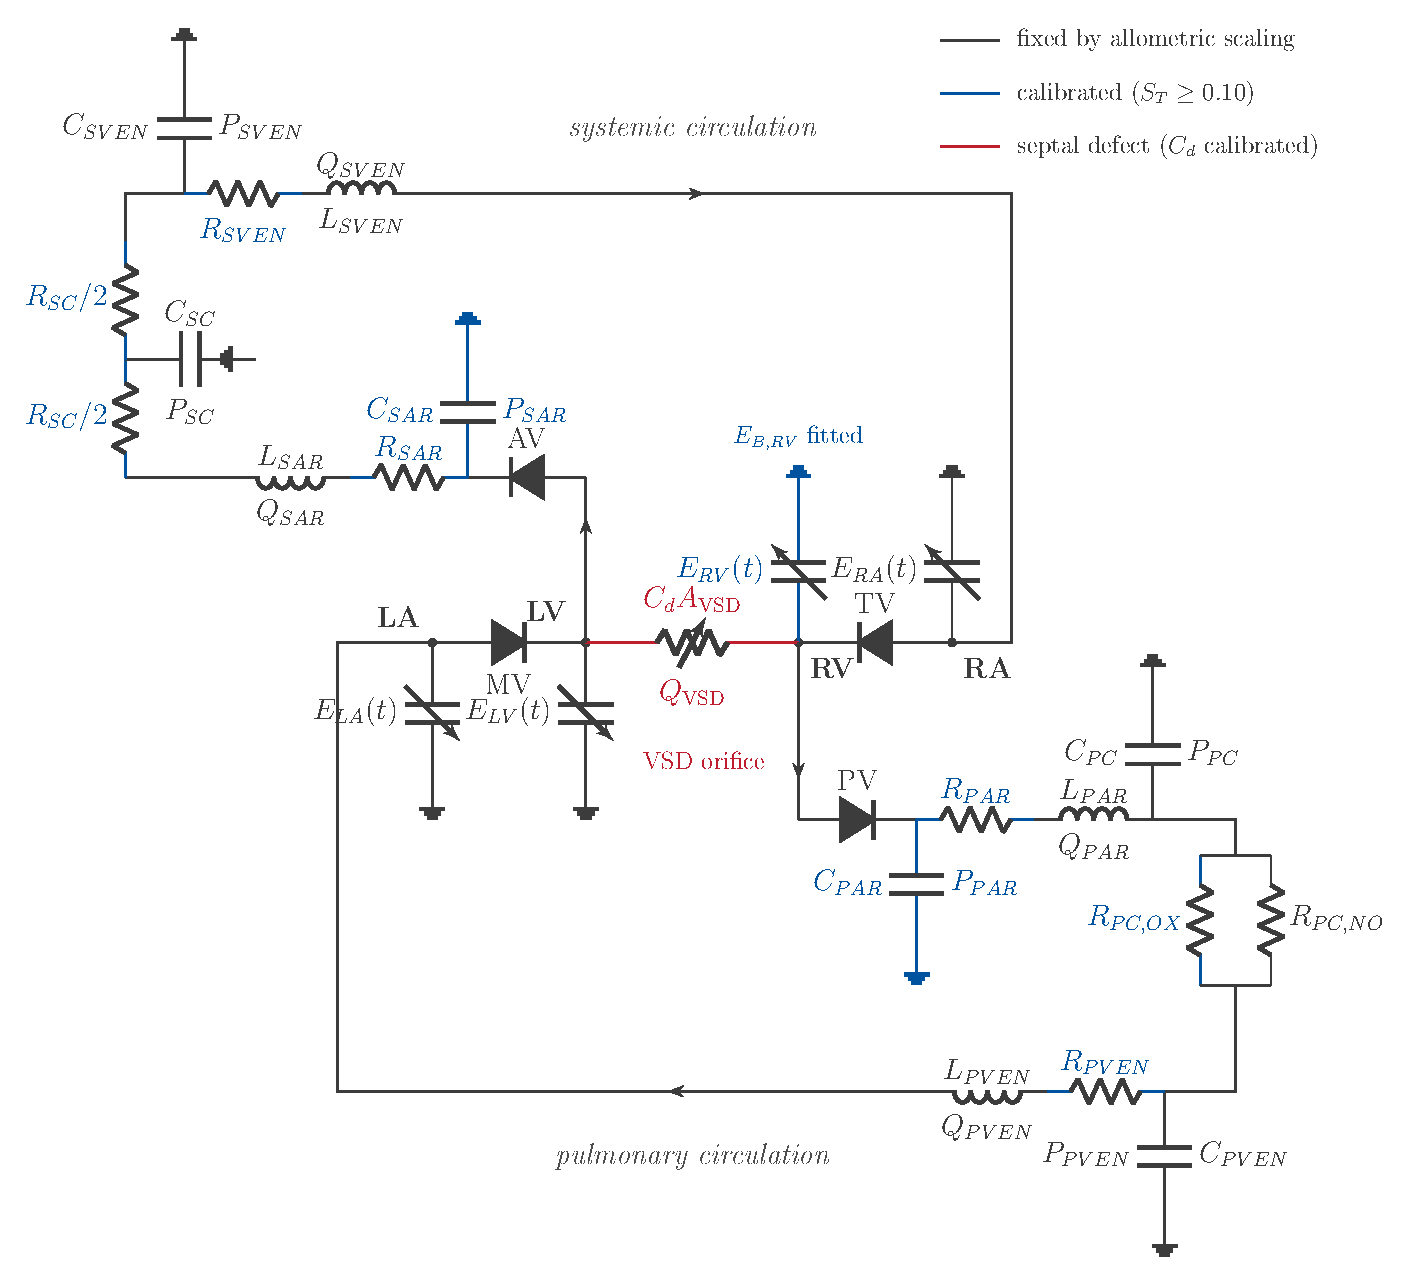
\includegraphics[width=\linewidth]{model_schematic.pdf}
\caption{Electrical analogue of the closed-loop model. Chambers are time-varying elastances, valves are smooth diodes, and the interventricular defect is a nonlinear orifice; $Q_{\mathrm{VSD}}$ is positive from LV to RV. $C_{\mathrm{PC}} = C_{\mathrm{PCOX}} + C_{\mathrm{PCNO}}$. Blue elements are calibrated, directly or through a resistance scale; $C_{\mathrm{SC}}$, $C_{\mathrm{SVEN}}$, $C_{\mathrm{PVEN}}$ and the oxygenated part of $C_{\mathrm{PC}}$ follow their resistance (Eq.~\ref{eq:rc}); all other elements are held at their allometrically scaled values. MV, AV, TV, PV: mitral, aortic, tricuspid and pulmonary valves.}
\label{fig:schematic}
\end{figure}

\FloatBarrier
\subsubsection{Cardiac chambers}
Chamber pressure follows the time-varying elastance model~\cite{Suga1974,Regazzoni2022},
\begin{equation}
P_{ch}(t) = E_{ch}(t)\left(V_{ch}(t) - V_{0,ch}\right), \qquad
E_{ch}(t) = E_{\mathrm{B},ch} + E_{\mathrm{A},ch}\, e_{ch}(t),
\label{eq:elastance}
\end{equation}
with unstressed volume $V_{0,ch}$, passive elastance $E_{\mathrm{B},ch}$, active elastance $E_{\mathrm{A},ch}$ and activation $e_{ch}(t)\in[0,1]$. Ventricular activation over the cardiac phase $\phi = \mathrm{mod}(t, T_{\mathrm{HB}})$, with $T_{\mathrm{HB}} = 60/\mathrm{HR}$, is the piecewise cosine of Regazzoni et al.~\cite{Regazzoni2022},
\begin{equation}
e_v(\phi) =
\begin{cases}
\tfrac{1}{2}\left[1-\cos\left(\pi\phi/T_{vc}\right)\right], & 0 \le \phi \le T_{vc},\\[3pt]
\tfrac{1}{2}\left[1+\cos\left(\pi(\phi-T_{vc})/T_{vr}\right)\right], & T_{vc} < \phi \le T_{vc}+T_{vr},\\[3pt]
0, & \text{otherwise},
\end{cases}
\label{eq:activation}
\end{equation}
where $T_{vc}$ and $T_{vr}$ are the contraction and relaxation durations. Atrial activation uses the same form with $\tau = \mathrm{mod}(\phi - t_{ac}, T_{\mathrm{HB}})$ in place of $\phi$ and the atrial durations $T_{ac}$ and $T_{ar}$, where $t_{ac}$ is the onset of atrial contraction. All timings are fixed fractions of $T_{\mathrm{HB}}$ (Appendix~\ref{app:nominal_parameters}), so they rescale with the measured heart rate of each state.

\FloatBarrier
\subsubsection{Valves and interventricular shunt}
\label{sec:valves}
Regazzoni et al.\ and Tonini et al.\ model each valve as a resistance that changes smoothly between an open and a closed value~\cite{Regazzoni2022,Tonini2025}. We use a tanh-gated conductance instead,
\begin{equation}
g = \tfrac{1}{2} + \tfrac{1}{2}\tanh\!\left(\frac{\Delta P}{\varepsilon_{\mathrm{v}}}\right), \qquad
Q_{\mathrm{valve}} = \Delta P\left(\frac{g}{R_{\mathrm{open}}} + \frac{1-g}{R_{\mathrm{closed}}}\right),
\label{eq:valve}
\end{equation}
with transvalvular gradient $\Delta P$ and $\varepsilon_{\mathrm{v}} = 0.5$~mmHg. The nominal resistances are $R_{\mathrm{open}} = 4.0\times10^{-3}$ and $R_{\mathrm{closed}} = 9.42\times10^{4}$~mmHg\,s/mL; after scaling (Section~\ref{sec:scaling}), $R_{\mathrm{open}} = 9.14\times10^{-3}$~mmHg\,s/mL for P1.

Valenti and Ferrero et al.\ represent the defect as a linear resistance~\cite{Valenti2023,Ferrero2026Shunts}. We replace it with the Gorlin orifice relation~\cite{Gorlin1951}, so that the shunt depends on the measured defect area, and add a sign-preserving factor that makes the relation differentiable at zero gradient,
\begin{equation}
Q_{\mathrm{VSD}} = 10^{6}\, C_d\, A_{\mathrm{VSD}} \sqrt{\frac{2\,\gamma\,\lvert\Delta P_{\mathrm{v}}\rvert}{\rho}}\;
\frac{\Delta P_{\mathrm{v}}}{\sqrt{\Delta P_{\mathrm{v}}^{2} + \varepsilon_{\mathrm{s}}^{2}}},
\qquad A_{\mathrm{VSD}} = \pi\left(\frac{D_{\mathrm{VSD}}}{2}\right)^{2},
\label{eq:orifice}
\end{equation}
where $Q_{\mathrm{VSD}}$ is in mL/s, $A_{\mathrm{VSD}}$ in m$^2$ (the factor $10^{6}$ converts m$^3$/s to mL/s), $\Delta P_{\mathrm{v}} = P_{\mathrm{LV}} - P_{\mathrm{RV}}$ in mmHg, $\gamma = 133.322$~Pa/mmHg, $\rho = 1060$~kg/m$^3$ and $\varepsilon_{\mathrm{s}} = 0.1$~mmHg. The discharge coefficient $C_d$ lumps the defect shape and the contraction of the jet; it is the only shunt parameter that is calibrated. Closure sets $A_{\mathrm{VSD}} = 0$, which gives $Q_{\mathrm{VSD}} = 0$ exactly.

\subsubsection{Coupling of compliance to resistance}
\label{sec:rc}
When calibration changes a resistance, the compliance of the same capillary or venous compartment is recomputed from it,
\begin{equation}
C_i = C_{i}^{\mathrm{s}}\,\min\!\left[\max\!\left(\left(\frac{R_i}{R_i^{\mathrm{s}}}\right)^{-4/3},\ 0.05\right),\ 8\right],
\qquad i \in \{\mathrm{SC},\,\mathrm{SVEN},\,\mathrm{PCOX},\,\mathrm{PVEN}\},
\label{eq:rc}
\end{equation}
where the superscript s denotes the allometrically scaled value. The relation is the resistance--compliance scaling of Corsini et al.~\cite{Corsini2014}, which follows from the dependence of vascular resistance and compliance on vessel length and radius~\cite{Pennati2000}. The arterial compliances $C_{\mathrm{SAR}}$ and $C_{\mathrm{PAR}}$ are calibrated directly and are not coupled. Equation~(\ref{eq:rc}) is applied during calibration and in every simulation that uses calibrated parameters; it is not applied in the sensitivity screen, where every input is sampled independently (Section~\ref{sec:gsa}).

\FloatBarrier
\subsection{Pediatric scaling and initialization}
\label{sec:scaling}

\subsubsection{Allometric scaling}
The adult reference parameters were scaled with the weight-based allometric law of Zhang et al.~\cite{zhang2019multiscale},
\begin{equation}
\theta_i = \theta_{i,\mathrm{ref}} \left(\frac{W_{\mathrm{p}}}{W_{\mathrm{ref}}}\right)^{\alpha_i},
\label{eq:scaling}
\end{equation}
with $W_{\mathrm{ref}} = 70$~kg, $W_{\mathrm{p}} = 13.4$~kg and the class exponents of Table~\ref{tab:exponents}. Zhang et al.\ give no exponent for inertance; we used $\alpha = -1$ from the mechanical-similarity argument of Lundquist et al.~\cite{Lundquist2025}. The age-dependent maturation of systemic and pulmonary resistance of Colebank et al.~\cite{Colebank2026} is implemented, but at the age of P1 (1158 days) both maturation factors equal 1.000. The scaled heart rate is replaced by the measured heart rate of each state.

\begin{table}[!htbp]
\centering\small
\caption{Weight-based allometric exponents used in Eq.~(\ref{eq:scaling}).}
\label{tab:exponents}
\begin{tabular}{llc}
\toprule
\textbf{Class} & \textbf{Parameters} & $\alpha_i$ \\
\midrule
Heart rate$^{\mathrm{a}}$ & HR & $-0.30$ \\
Left-heart elastance & $E_{\mathrm{A/B,LV}}$, $E_{\mathrm{A/B,LA}}$ & $-0.50$ \\
Right-heart elastance & $E_{\mathrm{A/B,RV}}$, $E_{\mathrm{A/B,RA}}$ & $-0.75$ \\
Systemic resistance & $R_{\mathrm{SAR}}$, $R_{\mathrm{SC}}$, $R_{\mathrm{SVEN}}$ & $-0.475$ \\
Pulmonary resistance & $R_{\mathrm{PAR}}$, $R_{\mathrm{PCOX}}$, $R_{\mathrm{PCNO}}$, $R_{\mathrm{PVEN}}$ & $-0.70$ \\
Compliance & all vascular $C$ & $+1.00$ \\
Unstressed volume & all $V_0$ & $+0.80$ \\
Inertance & all $L$ & $-1.00$\,$^{\mathrm{b}}$ \\
Valve open resistance & $R_{\mathrm{open}}$ & $-0.50$ \\
\bottomrule
\end{tabular}
\par\vspace{2pt}
\begin{minipage}{0.8\linewidth}
\raggedright\footnotesize
\emph{Note:} All exponents are from Zhang et al.~\cite{zhang2019multiscale} except $^{\mathrm{b}}$, from Lundquist et al.~\cite{Lundquist2025}. $^{\mathrm{a}}$Replaced by the measured heart rate of each state.
\end{minipage}
\end{table}

\subsubsection{Initial conditions and clinically seeded parameters}
Table~\ref{tab:seeding} lists every initial condition and every parameter seeded from the clinical record, with its formula and value for P1. The total blood volume is $\mathrm{BV} = 70$~mL/kg~$\times\,W_{\mathrm{p}} = 938$~mL, the standard estimate for children older than three years~\cite{Cote2024}. The systemic venous unstressed volume closes the volume budget,
\begin{equation}
V_{0,\mathrm{SVEN}} = \mathrm{BV} - \sum_{i \neq \mathrm{SVEN}} V_i(0) - P_{\mathrm{nom,SVEN}}\,C_{\mathrm{SVEN}},
\label{eq:sven}
\end{equation}
where the sum runs over the four chambers and the other eight vascular volume states, bounded to $[\max(0.01\,\mathrm{BV},\,1~\mathrm{mL}),\ 0.85\,\mathrm{BV}]$. The vascular resistances start at their scaled values, because neither SVR nor PVR was recorded on the protocol form.

\begin{table}[!htbp]
\centering\small
\setlength{\tabcolsep}{4pt}
\caption{Initial conditions and clinically seeded parameters for P1. $P_{\mathrm{nom}}$ is the nominal compartment pressure used to place the initial volume.}
\label{tab:seeding}
\resizebox{\linewidth}{!}{\begin{tabular}{llll}
\toprule
\textbf{Quantity} & \textbf{Definition} & \textbf{Formula} & \textbf{Value} \\
\midrule
\multicolumn{4}{l}{\emph{Initial conditions}} \\
BV & total blood volume & $70$~mL/kg $\times\,W_{\mathrm{p}}$ & 938 mL \\
$V_i(0)$, vascular & initial vascular volume & $V_{0,i} + P_{\mathrm{nom},i}\,C_i$ & -- \\
$V_{ch}(0)$ & initial chamber volume & $V_{0,ch} + P_{\mathrm{ED},ch}/E_{\mathrm{B},ch}$ & -- \\
$P_{\mathrm{nom,SAR}}$ & systemic arterial & mean arterial pressure & 71.33 mmHg \\
$P_{\mathrm{nom,SC}}$ & systemic capillary & $\max(0.5\,P_{\mathrm{nom,SAR}},\,15)$ & 35.7 mmHg \\
$P_{\mathrm{nom,SVEN}}$, $P_{\mathrm{ED,RA}}$, $P_{\mathrm{ED,RV}}$ & venous and right-heart filling & mean RA pressure & 5 mmHg \\
$P_{\mathrm{nom,PAR}}$ & pulmonary arterial & mean PA pressure & 15 mmHg \\
$P_{\mathrm{nom,PVEN}}$, $P_{\mathrm{ED,LA}}$, $P_{\mathrm{ED,LV}}$ & left-heart filling & assumed (LA pressure not measured) & 6 / 6 / 8 mmHg \\
$P_{\mathrm{PC}}(0)$ & pulmonary capillary & $(P_{\mathrm{nom,PAR}}+P_{\mathrm{nom,PVEN}})/2$ & 10.5 mmHg \\
\midrule
\multicolumn{4}{l}{\emph{Clinically seeded parameters}} \\
$C_{\mathrm{SAR}}$ & systemic arterial compliance & $(Q_s/\mathrm{HR})/(P_{\mathrm{sys}}-P_{\mathrm{dia}})_{\mathrm{RFA}}$ & 0.669 mL/mmHg \\
$C_{\mathrm{PAR}}$ & pulmonary arterial compliance & $(Q_p/\mathrm{HR})/(P_{\mathrm{sys}}-P_{\mathrm{dia}})_{\mathrm{PA}}$ & 3.434 mL/mmHg \\
$C_d$ & discharge coefficient & Eq.~(\ref{eq:orifice}) solved for $C_d$ at $Q_{\mathrm{shunt}}$ and $\Delta P_{\mathrm{v}} = \tfrac12 \Delta P_{\mathrm{LV-RV,peak}}$ & 0.356 \\
\bottomrule
\end{tabular}}
\par\vspace{2pt}
\begin{minipage}{0.97\linewidth}
\raggedright\footnotesize
\emph{Note:} $C_{\mathrm{SAR}}$ and $C_{\mathrm{PAR}}$ are set to stroke volume over pulse pressure, following Colebank et al.~\cite{Colebank2026}. The $C_d$ seed uses half of the measured peak LV--RV systolic gradient (69~mmHg) as a representative gradient over the cycle; this choice is ours.
\end{minipage}
\end{table}

\FloatBarrier
\subsection{Numerical solution}
\label{sec:numerics}
The system was integrated with \texttt{ode15s}~\cite{Shampine1997} in MATLAB R2025a, with relative tolerance $10^{-5}$, absolute tolerance $10^{-6}$, maximum step $T_{\mathrm{HB}}/20$ and the sparsity pattern of the Jacobian supplied. The solver advanced the model in batches of five cardiac cycles and compared the peak value of each state between consecutive batches. Periodic steady state was declared when every volume state changed by less than 0.1~mL, $P_{\mathrm{PC}}$ by less than 0.1~mmHg and every flow state by less than 0.5\% of its peak (0.1~mL/s when the peak was below 0.1~mL/s), within at most 80 cycles. Outputs were computed from the last two cycles. During calibration, each simulation was limited to 30--60 cycles with a steady-state tolerance of 0.5~mL and 0.5~mmHg to reduce cost, and a simulation that did not reach steady state added a penalty of $10^{3}$ to the objective. The scaled baseline, the calibrated pre-closure state and the post-closure prediction were recomputed with the full settings and reached steady state; the post-closure cycle closes to within 0.03~mL in every volume state. The atrial and systemic and pulmonary venous pressures are bounded below at $-5$~mmHg to avoid solver failure from non-physiological initial states; the bound is not active in the reported states, where the lowest atrial pressure is 2.9~mmHg and the lowest venous pressure 8.5~mmHg. We verified the reported pre-closure and post-closure states numerically (Supplementary Section~S4). Tightening the tolerances tenfold and a hundredfold changed no output by more than 0.07\%, reducing the maximum step to $T_{\mathrm{HB}}/50$ changed no output, and running 20 further cycles after steady state changed no output by more than 0.05\%. Total blood volume is conserved over the cycle to within $10^{-4}$~mL.

\FloatBarrier
\subsection{Global sensitivity analysis}
\label{sec:gsa}
Variance-based global sensitivity analysis~\cite{Sobol2001,Saltelli2010} ranked the parameters by their influence on the model outputs, following recommendations for cardiovascular models~\cite{Eck2016} and the approach of Tonini et al.\ for this model~\cite{Tonini2025}. We fitted sparse polynomial chaos expansions (PCE)~\cite{Blatman2011} in UQLab~2.2~\cite{Marelli2014} (least-angle regression, degree 1--3, hyperbolic truncation $q = 0.75$) to one Halton design of $N = 128$ points over $d = 21$ independent uniform inputs. The input ranges were $[0.4,\,2.5]\,x_0$ for resistances, $[0.5,\,2.0]\,x_0$ for compliances and elastances, $[0.6,\,1.7]\,x_0$ for unstressed volumes and $[0.8,\,1.2]\,x_0$ for $C_d$, where $x_0$ is the scaled and seeded value. The total-order Sobol' index of each input,
\begin{equation}
S_{T_i} = 1 - \frac{\mathrm{Var}\!\left(\mathbb{E}\left[Y \mid \mathbf{X}_{\sim i}\right]\right)}{\mathrm{Var}(Y)},
\label{eq:sobol}
\end{equation}
was computed analytically from the expansion coefficients~\cite{Sudret2008} for 25 outputs. All 128 training simulations completed.

The 21 inputs contain the 14 calibration candidates. The systemic resistance scale multiplies $R_{\mathrm{SAR}}$ and $R_{\mathrm{SC}}$, and the pulmonary resistance scale multiplies $R_{\mathrm{PAR}}$, $R_{\mathrm{PCOX}}$ and $R_{\mathrm{PVEN}}$; each scale takes the largest index of its members. The other four inputs, $C_{\mathrm{SVEN}}$, $C_{\mathrm{PVEN}}$, $V_{0,\mathrm{LA}}$ and $V_{0,\mathrm{RA}}$, are not calibration candidates: the two venous compliances follow their resistances during calibration (Eq.~\ref{eq:rc}), and the atrial unstressed volumes were held at their scaled values. A candidate was retained if $S_{T} \ge 0.10$ for at least one of the nine calibration targets (Section~\ref{sec:comparison}), the threshold Valenti used to select calibration parameters in patients with septal defects~\cite{Valenti2023}. The screen fixes the calibrated parameter set; no later stage adds a parameter.

To keep the design affordable, each training simulation ran for at most 10 cycles with a steady-state tolerance of 1.0~mmHg and 1.0~mL, and outputs were taken from cycles 9--10. The screen was repeated at the calibrated operating point with the same relative input ranges. With 128 points, the indices are used to rank the parameters, not as precise values.

\FloatBarrier
\subsection{Calibration}
\label{sec:calibration}

\subsubsection{Objective function}
Calibration minimized
\begin{equation}
J(\mathbf{x}) = \sum_{k \in \mathcal{P}} w_k\left(\frac{\varepsilon_k}{0.05}\right)^{2}
+ \sum_{k \in \mathcal{S}} w_k\left(\frac{\varepsilon_k}{0.10}\right)^{2}
+ J_{\mathrm{sys}} + J_{\mathrm{shape}} + J_{\mathrm{shunt}} + J_{\mathrm{guard}}
+ J_{\mathrm{gate}} + J_{\mathrm{prior}} + J_{\mathrm{bound}} + J_{\mathrm{range}},
\label{eq:objective}
\end{equation}
with the signed relative error $\varepsilon_k = (y_k(\mathbf{x}) - y_k^{\mathrm{clin}})/y_k^{\mathrm{clin}}$ and the target weights $w_k$ of Supplementary Table~S3. The terms are:
\begin{itemize}[leftmargin=1.5em,itemsep=1pt]
\item $\mathcal{P}$: mean PA pressure and $Q_p/Q_s$; $\mathcal{S}$: systolic and diastolic PA and RFA pressure and shunt flow.
\item $J_{\mathrm{sys}}$: mean RA pressure, mean arterial pressure and $Q_s$ enter together, each as $(\Delta y/\sigma)^2$ with its declared uncertainty $\sigma$, so that one systemic mismatch is not counted three times; it adds a one-sided penalty when $Q_s$ falls below $Q_s^{\mathrm{clin}} - \sigma_{Q_s}$ and a penalty on the difference between aortic and systemic flow.
\item $J_{\mathrm{shape}}$: systolic and diastolic RFA pressure and the systemic and pulmonary pulse pressures, each normalized by 0.10.
\item $J_{\mathrm{shunt}}$: the difference between the cycle-mean orifice flow and $Q_p - Q_s$, and between $Q_p - Q_s$ and the clinical shunt flow.
\item $J_{\mathrm{guard}}$: a quadratic penalty when the relative error of systolic or diastolic RFA or PA pressure or of mean PA pressure exceeds 12\%, and a second one when the error of mean PA pressure exceeds 8\%.
\item $J_{\mathrm{gate}}$: $\lambda_{\mathrm{g}}\sum_{k}[\max(0,\lvert\varepsilon_k\rvert - 0.10)/0.10]^2$ over the nine calibration targets, $\lambda_{\mathrm{g}} = 20$.
\item $J_{\mathrm{prior}}$: $\lambda_{\mathrm{p}}\sum_{j} c_j \ln^{2}(x_j/x_j^{\mathrm{s}})$, the drift from the scaled value, with confidence weight $c_j = 2.0$ for $C_{\mathrm{SAR}}$ and $C_{\mathrm{PAR}}$ and 1.0 for the other five parameters, and $\lambda_{\mathrm{p}} = 0.375$.
\item $J_{\mathrm{bound}}$: $\lambda_{\mathrm{b}}\sum_{j}[\max(0, 0.10 - d_j)]^2$, where $d_j$ is the distance of $x_j$ to the nearer bound as a fraction of the bound interval, $\lambda_{\mathrm{b}} = 17$.
\item $J_{\mathrm{range}}$: a penalty on outputs without a clinical value (chamber volumes, ejection fractions, PVR) that leave pediatric physiological ranges, with weight 50 outside the soft range and 400 outside the hard range (Supplementary Table~S4), plus a penalty for simulations that are not physiologically valid or do not reach steady state.
\end{itemize}
The full definition of each term is given in Supplementary Section~S3. The objective and its weights are specific to this work.

\subsubsection{Bounds}
Each calibrated parameter has a lower and an upper bound (Table~\ref{tab:bounds}): $[0.25,\,2.8]$ for the systemic and $[0.45,\,2.8]$ for the pulmonary resistance scale; $[0.40,\,2.8]$ and $[0.55,\,2.6]$ times the scaled value for $R_{\mathrm{SVEN}}$ and $E_{\mathrm{B,RV}}$; $[0.75,\,1.35]$ and $[0.70,\,1.45]$ times the clinical seed for $C_{\mathrm{SAR}}$ and $C_{\mathrm{PAR}}$, with the lower bound extended to just below the scaled value (the scaled value minus 5\% of it or 2\% of the interval, whichever is larger) so that the scaled value stays feasible; and $[0.8\times$ seed, $1.05\times$ adult reference$]$ for $C_d$. We chose these bounds to cover the physiological range of each parameter class around its scaled or seeded value; they are not taken from a published source. Supplementary Table~S5 lists every bound with the scaled and seeded value.

\subsubsection{Staged multi-start optimization}
For each starting point, six bound-constrained subproblems were solved in sequence with \texttt{fmincon} (Table~\ref{tab:stages}). Stages A--E used the interior-point algorithm with a limited-memory BFGS Hessian, forward finite differences with step $10^{-5}$, optimality tolerance $10^{-5}$, step tolerance $10^{-6}$, and at most 300 function evaluations and 40 iterations. Stage F used sequential quadratic programming on a separate score that penalizes each calibration target with a relative error above 10\% (forward finite differences with step $10^{-4}$, at most 900 function evaluations and 120 iterations, two starts: the current point and the clinical seed). Stages D, E and F were kept only if they passed the acceptance rule in Table~\ref{tab:stages}.

\begin{table}[!htbp]
\centering\small
\setlength{\tabcolsep}{3pt}
\caption{Calibration stages for each starting point.}
\label{tab:stages}
\resizebox{\linewidth}{!}{\begin{tabular}{llll}
\toprule
\textbf{Stage} & \textbf{Free parameters} & \textbf{Targets} & \textbf{Kept if} \\
\midrule
A & $R_{\mathrm{sys}}$, $R_{\mathrm{SVEN}}$, $R_{\mathrm{pul}}$, $C_{\mathrm{SAR}}$, $C_{\mathrm{PAR}}$, $C_d$ & RA, RFA and mean PA pressure, $Q_p/Q_s$, $Q_s$, shunt flow & always \\
B & $E_{\mathrm{B,RV}}$ & mean RA pressure & always \\
C & all seven & all calibration targets & always \\
D & $R_{\mathrm{sys}}$, $R_{\mathrm{SVEN}}$, $C_{\mathrm{SAR}}$, $E_{\mathrm{B,RV}}$ & mean arterial, RA and PA pressure, $Q_s$, $Q_p/Q_s$ & RMSE and number of mean-pressure and flow targets above 10\% do not increase \\
E & all seven, $\lambda_{\mathrm{p}} = 2.25$, $\lambda_{\mathrm{b}} = 120$ & all calibration targets & fewer plausibility warnings; RMSE rises by $< 0.005$ \\
F & all seven (SQP, gate score) & all calibration targets & RMSE or number of targets above 10\% falls \\
\bottomrule
\end{tabular}}
\end{table}

Six starting points were used: the clinical seed and five points of a scrambled Sobol' sequence (Matou\v{s}ek affine--Owen scrambling, first point skipped) mapped uniformly into the bounds, generated with the seed 101, fixed in advance. One result was selected in three ordered steps: fewest of the five mean-pressure and flow targets with a relative error above 10\%, then fewest of the nine calibration targets above 10\%, then lowest RMSE. The 10\% value in the objective and in this rule is an internal setting of the optimizer; the Results report the relative errors and apply no threshold. Repeating the pipeline with the seeds 202 and 303 returned the same parameter set (Supplementary Section~S1).

\FloatBarrier
\subsection{Post-closure prediction}
\label{sec:post_methods}
The post-closure state is a prediction, not a fit. The calibrated pre-closure parameters, including the compliances set by Eq.~(\ref{eq:rc}), were applied unchanged with the defect closed ($A_{\mathrm{VSD}} = 0$) and the heart rate set to its post-closure value (108~bpm), which rescales all chamber timings. No parameter was refitted and no post-closure measurement entered calibration. The prediction therefore represents the circulation immediately after closure, with the chamber properties of the pre-closure state.

\FloatBarrier
\subsection{Comparison between model and measurements}
\label{sec:comparison}
\label{sec:statistics}
Every measured quantity is reported with its measured value, the model value and the relative error $\varepsilon_k$, in the same order and with the same symbols before and after closure. Where an uncertainty is declared, the standardized residual $z_k = (y_k^{\mathrm{model}} - y_k^{\mathrm{clin}})/\sigma_k$ is also given, with $\sigma_k$ the one-standard-deviation uncertainty: 5\% of the measured value for catheter RA and PA pressures, mean arterial pressure and $Q_p/Q_s$; 10\% for systolic and diastolic systemic pressure, ventricular volumes and ejection fractions; 0.50~L/min (14.6\%) for pre-closure $Q_s$; 5\% for post-closure $Q_s$; and 20\% for derived quantities (shunt flow, SVR). The 14.6\% for Fick-derived $Q_s$ is close to the standard deviation of Fick output against thermodilution or MRI in children when oxygen consumption is measured (17.3\%)~\cite{Ralston2023}. The 5\% for catheter RA and PA pressures matches the spread of the repeated readings on the protocol form (at most 1~mmHg), and the 10\% for systolic and diastolic systemic pressure matches the 9~mmHg difference between the RFA and descending-aortic systolic readings. The other values are our assumptions.

The nine calibration targets are mean RA pressure, mean, systolic and diastolic PA pressure, mean, systolic and diastolic RFA pressure, $Q_s$ and $Q_p/Q_s$. In both states they are summarized by the root-mean-square of their relative errors,
\begin{equation}
\mathrm{RMSE} = \sqrt{\frac{1}{9}\sum_{k=1}^{9}\varepsilon_k^{2}}.
\label{eq:rmse}
\end{equation}
Shunt flow is a calibration target but is excluded from the RMSE because it is the difference of two calibrated flows. No acceptance threshold is applied to any result.

Ventricular pressure--volume loops were characterized by end-diastolic volume (maximum volume), end-systolic volume (minimum volume), stroke volume, ejection fraction, end-diastolic pressure (pressure at maximum volume), end-systolic pressure (pressure at the maximum of $P/V$), peak pressure and stroke work, $\mathrm{SW} = \oint P\,dV$. End-systolic pressure is taken at the maximum of $P/V$ because, with an open defect, the LV keeps emptying into the RV during relaxation and reaches its minimum volume after pressure has fallen. Because one patient was studied, no between-patient statistics were computed. The practical identifiability of the calibrated parameters is reported in Supplementary Section~S2.

\FloatBarrier
\subsection{Measurement-noise simulation}
\label{sec:noise_methods}
The effect of measurement uncertainty on the calibrated parameters and on the post-closure prediction was assessed by Monte Carlo simulation. In each of $M = 20$ replicates, every directly measured pre-closure target was perturbed independently by zero-mean Gaussian noise with standard deviation $\sigma_k$ (Section~\ref{sec:comparison}): mean RA pressure (0.25~mmHg), mean, systolic and diastolic PA pressure (0.75, 1.0 and 0.5~mmHg), systolic and diastolic RFA pressure (10 and 5.7~mmHg), $Q_s$ (0.50~L/min) and $Q_p/Q_s$ (0.060). Mean arterial pressure and shunt flow were recomputed from the perturbed values with the formulas of Section~\ref{sec:data}. A draw was redrawn only if it was physically impossible: a non-positive value, diastolic above systolic pressure, mean PA pressure outside its systolic--diastolic range, or $Q_p/Q_s \le 1$. Model inputs (age, weight, heart rate, defect diameter) and all post-closure measurements were not perturbed. The draws used a fixed seed (20260926) and were generated in sequence, so the $M$ replicates are the first $M$ draws of that stream. $M$ was set to 20 because each recalibration takes about 85~min; with $M = 20$ the standard deviation across replicates has a relative standard error of about 16\%.

Each perturbed record was recalibrated with the procedure of Section~\ref{sec:calibration} unchanged: the same seeding, objective, six starting points and multi-start seed, and the same seven parameters, so that only the measurements differ between replicates. A replicate whose seeded $C_d$ fell outside its bounds could not be calibrated; it is reported as such and excluded from the statistics. The recalibrated parameters were applied with the defect closed, as in Section~\ref{sec:post_methods}, and the prediction was compared with the unperturbed post-closure record. For each calibrated parameter and each predicted quantity we report the mean, standard deviation, coefficient of variation and range (minimum to maximum) across replicates.

\FloatBarrier
\subsection{Implementation}
The model, calibration and analyses were implemented in MATLAB R2025a (MathWorks, Natick, MA) with the Optimization and the Statistics and Machine Learning Toolboxes and UQLab~2.2~\cite{Marelli2014}; figures were drawn in R~4.5.2 with ggplot2. One calibration took about 85~min on a laptop with an AMD Ryzen~5 5600H processor and 16~GB of RAM. One script (\texttt{run\_all.m}) reproduces the pre-closure pipeline, the post-closure prediction and every exported table, and a second (\texttt{run\_noise\_simulation.m}) reproduces the measurement-noise simulation.

% =====================================================================
\FloatBarrier
\section{Results}
\label{sec:results}

\subsection{Sensitivity analysis}
\label{sec:results_gsa}
The screen retained 7 of the 14 candidate parameters (Figure~\ref{fig:gsa}A). Ranked by their largest total-order index over the nine fitted targets, the retained parameters were the systemic resistance scale ($S_T = 0.70$), the discharge coefficient $C_d$ (0.51), the passive right-ventricular elastance $E_{\mathrm{B,RV}}$ (0.48), the pulmonary resistance scale (0.40), the pulmonary arterial compliance $C_{\mathrm{PAR}}$ (0.39), the systemic arterial compliance $C_{\mathrm{SAR}}$ (0.12) and the systemic venous resistance $R_{\mathrm{SVEN}}$ (0.10). The other seven candidates stayed below 0.10 for every fitted target: $E_{\mathrm{A,RV}}$ (0.080), $E_{\mathrm{B,LV}}$ (0.073), $E_{\mathrm{A,LV}}$ (0.031), $E_{\mathrm{A,RA}}$ (0.006), $E_{\mathrm{A,LA}}$ (0.005), $V_{0,\mathrm{RV}}$ (0.004) and $V_{0,\mathrm{LV}}$ (0.001).

Each fitted target was controlled by one or two parameters (Figure~\ref{fig:gsa}B). The systemic resistance scale controlled diastolic RFA pressure ($S_T = 0.70$), mean arterial pressure (0.58), systolic RFA pressure (0.43), $Q_p/Q_s$ (0.41) and systemic flow (0.33). $C_d$ controlled $Q_p/Q_s$ (0.51). $E_{\mathrm{B,RV}}$ controlled mean RA pressure (0.48). The pulmonary resistance scale controlled diastolic and mean PA pressure (0.40 and 0.30), and $C_{\mathrm{PAR}}$ controlled systolic PA pressure (0.39). At the calibrated operating point (Supplementary Figure~S2), the dominant parameter was the same for eight of the nine targets. For systolic PA pressure, the pulmonary resistance scale became dominant ($S_T = 0.25$) and $C_{\mathrm{PAR}}$ fell to 0.06; calibration lowered $C_{\mathrm{PAR}}$ from its seed of 3.43 to 1.02~mL/mmHg, which narrows the absolute range sampled around it.

The parameters left out by the screen controlled the chamber outputs that have no pre-closure measurement: $E_{\mathrm{A,LV}}$ controlled LVESV ($S_T = 0.59$) and LVEF (0.63), and $E_{\mathrm{A,RV}}$ controlled RVESV (0.71) and RVEF (0.76). Of the four screened inputs that are not calibration candidates, $C_{\mathrm{SVEN}}$ exceeded 0.10 for five fitted targets (largest 0.14, diastolic PA pressure) and reached 0.18 for systolic PA pressure at the calibrated operating point; $C_{\mathrm{PVEN}}$ stayed below 0.03 at the baseline and reached 0.14 at the calibrated operating point; $V_{0,\mathrm{LA}}$ and $V_{0,\mathrm{RA}}$ stayed below 0.01. $C_{\mathrm{SVEN}}$ was therefore not calibrated directly although its influence exceeded the retention threshold; during calibration it followed $R_{\mathrm{SVEN}}$ through Eq.~(\ref{eq:rc}) and fell from 5.74 to 3.32~mL/mmHg. The polynomial chaos expansions had modified leave-one-out errors of 0.043--0.155 across the 25 outputs. All 256 training simulations of the two screens reached the 10-cycle limit before meeting the 1.0~mmHg / 1.0~mL tolerance, so the indices describe outputs from cycles 9--10 of each training simulation.

\begin{figure}[!htbp]
\centering
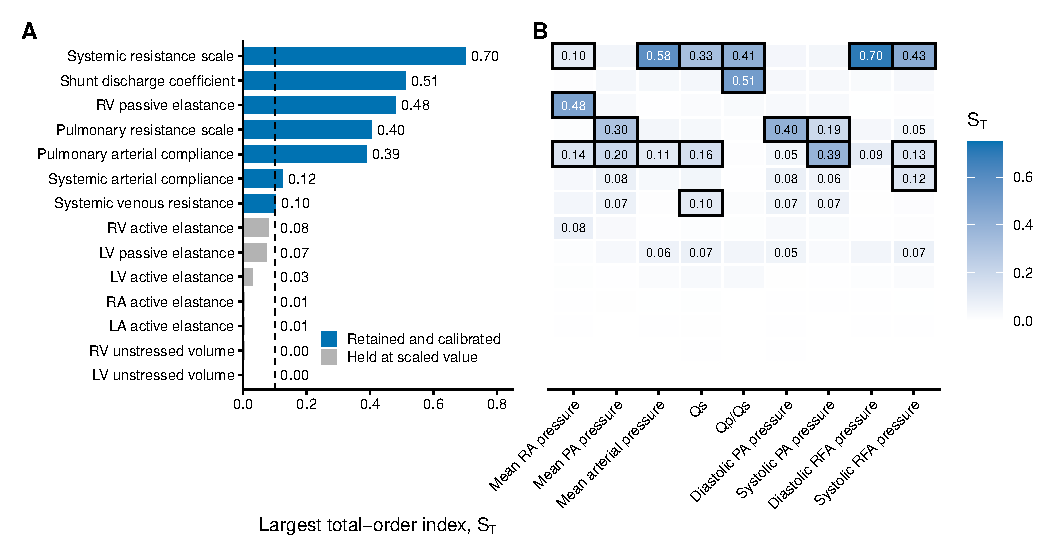
\includegraphics[width=0.92\linewidth]{M1_gsa_screening.pdf}
\caption{Global sensitivity screen at the scaled baseline. (A) Largest total-order Sobol' index of each calibration candidate over the nine fitted targets; the dashed line is the retention threshold $S_T = 0.10$. (B) Total-order index of every candidate for every fitted target; blank cells are below 0.005.}
\label{fig:gsa}
\end{figure}

\FloatBarrier
\subsection{Pre-closure calibration}
\label{sec:results_pre}
Table~\ref{tab:pre_targets} lists every pre-closure measurement beside the scaled baseline and the calibrated model. Calibration reduced the RMSE of relative error over the nine fitted targets from 0.274 to 0.105. Systolic PA pressure had the largest standardized residual ($z = +5.10$); every other calibration target had $\lvert z\rvert \le 1.27$.

The relative errors of the calibrated model for the fitted targets were $+4.6\%$ for mean RA pressure, $+5.5\%$ for mean PA pressure, $-3.0\%$ for diastolic PA pressure, $+25.5\%$ for systolic PA pressure (25.1 against 20~mmHg), $-2.5\%$ for mean arterial pressure, $-7.5\%$ for diastolic RFA pressure, $-11.9\%$ for systolic RFA pressure (88.1 against 100~mmHg), $-8.0\%$ for $Q_s$ and $-3.1\%$ for $Q_p/Q_s$. Shunt flow was 0.496 against 0.664~L/min ($-25.3\%$).

For the measurements that were not fitted, the relative errors were $-5.3\%$ for LV systolic pressure, $+6.7\%$ for RV systolic pressure, $-9.7\%$ for the LV--RV systolic gradient, $-3.2\%$ and $-7.5\%$ for DAo systolic and diastolic pressure, $-10.8\%$ for $Q_p$ and $+5.4\%$ for SVR. The cuff pressure recorded in the same session (119/83~mmHg) was 19 and 26~mmHg above the RFA catheter readings and 26.0\% and 36.4\% above the model.

\begin{table}[!htbp]
\centering\small
\setlength{\tabcolsep}{3pt}
\caption{Pre-closure record against the scaled baseline and the calibrated model. $\sigma$, declared uncertainty; $\varepsilon$, relative error; $z = (\text{model}-\text{measured})/\sigma$ for the calibrated model; --, not measured or not defined. The three multi-start seeds give identical values.}
\label{tab:pre_targets}
\resizebox{\linewidth}{!}{\begin{tabular}{lcrrrrrrr}
\toprule
\textbf{Quantity} & \textbf{Fitted} & $\sigma$ & \textbf{Measured} & \textbf{Baseline} & $\varepsilon$ (\%) & \textbf{Calibrated} & $\varepsilon$ (\%) & $z$ \\
\midrule
\multicolumn{9}{l}{\emph{Systemic arterial pressure}} \\
Systolic pressure, RFA (mmHg) & yes & 10.0 & 100.00 & 88.19 & $-11.8$ & 88.09 & $-11.9$ & $-1.19$ \\
Diastolic pressure, RFA (mmHg) & yes & 5.70 & 57.00 & 65.75 & $+15.4$ & 52.75 & $-7.5$ & $-0.75$ \\
Mean arterial pressure, RFA (mmHg) & yes & 3.57 & 71.33 & 77.04 & $+8.0$ & 69.56 & $-2.5$ & $-0.50$ \\
Systolic pressure, DAo (mmHg) & no & -- & 91.00 & 88.19 & $-3.1$ & 88.09 & $-3.2$ & -- \\
Diastolic pressure, DAo (mmHg) & no & -- & 57.00 & 65.75 & $+15.4$ & 52.75 & $-7.5$ & -- \\
Systolic pressure, cuff (mmHg) & no & -- & 119.00 & 88.19 & $-25.9$ & 88.09 & $-26.0$ & -- \\
Diastolic pressure, cuff (mmHg) & no & -- & 83.00 & 65.75 & $-20.8$ & 52.75 & $-36.4$ & -- \\
\multicolumn{9}{l}{\emph{PA and RA pressure}} \\
PA systolic pressure (mmHg) & yes & 1.00 & 20.00 & 21.41 & $+7.1$ & 25.10 & $+25.5$ & $+5.10$ \\
PA diastolic pressure (mmHg) & yes & 0.50 & 10.00 & 16.50 & $+65.0$ & 9.70 & $-3.0$ & $-0.60$ \\
Mean PA pressure (mmHg) & yes & 0.75 & 15.00 & 19.05 & $+27.0$ & 15.82 & $+5.5$ & $+1.09$ \\
Mean RA pressure (mmHg) & yes & 0.25 & 5.00 & 5.05 & $+1.1$ & 5.23 & $+4.6$ & $+0.93$ \\
\multicolumn{9}{l}{\emph{Ventricular pressure}} \\
LV systolic pressure (mmHg) & no & -- & 94.0 & 88.6 & $-5.7$ & 89.0 & $-5.3$ & -- \\
RV systolic pressure (mmHg) & no & -- & 25.0 & 22.6 & $-9.7$ & 26.7 & $+6.7$ & -- \\
LV--RV systolic gradient (mmHg) & no & -- & 69.0 & 66.0 & $-4.3$ & 62.3 & $-9.7$ & -- \\
\multicolumn{9}{l}{\emph{Flow and resistance}} \\
Pulmonary flow $Q_p$ (L/min) & no & -- & 4.087 & 2.629 & $-35.7$ & 3.645 & $-10.8$ & -- \\
Systemic flow $Q_s$ (L/min) & yes & 0.50 & 3.423 & 2.188 & $-36.1$ & 3.149 & $-8.0$ & $-0.55$ \\
$Q_p/Q_s$ (--) & yes & 0.060 & 1.194 & 1.201 & $+0.6$ & 1.157 & $-3.1$ & $-0.61$ \\
Shunt flow $Q_p - Q_s$ (L/min) & yes & 0.133 & 0.664 & 0.441 & $-33.7$ & 0.496 & $-25.3$ & $-1.27$ \\
SVR (WU) & no & -- & 19.38 & 32.90 & $+69.8$ & 20.43 & $+5.4$ & -- \\
\multicolumn{9}{l}{\emph{Ventricular volume and function}} \\
LVEDV (mL) & no & -- & -- & 31.8 & -- & 39.8 & -- & -- \\
LVESV (mL) & no & -- & -- & 10.0 & -- & 9.8 & -- & -- \\
RVEDV (mL) & no & -- & -- & 34.2 & -- & 43.3 & -- & -- \\
RVESV (mL) & no & -- & -- & 13.8 & -- & 14.9 & -- & -- \\
LVEF (--) & no & -- & -- & 0.69 & -- & 0.75 & -- & -- \\
RVEF (--) & no & -- & -- & 0.60 & -- & 0.65 & -- & -- \\
\midrule
RMSE of $\varepsilon$, nine fitted targets & & & & 0.274 & & 0.105 & & \\
$\chi^2/N$, nine fitted targets ($N=9$) & & & & 23.62 & & 3.48 & & \\
\bottomrule
\end{tabular}}
\end{table}

Two of the seven calibrated parameters converged onto their lower bounds (Table~\ref{tab:bounds}): the pulmonary resistance scale (0.450, lower bound 0.450) and $E_{\mathrm{B,RV}}$ (0.0799~mmHg/mL, lower bound 0.0798). The objective therefore preferred values below the lower bound of both parameters. Of the parameters that moved freely, the systemic resistance scale fell to 0.57 of its scaled value, $C_{\mathrm{SAR}}$ rose to 2.24 times and $R_{\mathrm{SVEN}}$ to 1.51 times its scaled value, $C_{\mathrm{PAR}}$ stayed at 1.06 times, and $C_d$ settled at 0.370, 4\% above its clinically seeded value of 0.356 and 47\% below the adult reference of 0.70.

\begin{table}[!htbp]
\centering\small
\setlength{\tabcolsep}{4pt}
\caption{The seven calibrated parameters: allometrically scaled value, clinically seeded start, bounds, calibrated value and ratio to the scaled value. Resistance scales are dimensionless multipliers of the scaled compartment resistances.}
\label{tab:bounds}
\resizebox{\linewidth}{!}{\begin{tabular}{llrrrrrr}
\toprule
\textbf{Parameter} & \textbf{Unit} & \textbf{Scaled} & \textbf{Seed} & \textbf{Lower} & \textbf{Upper} & \textbf{Calibrated} & \textbf{Ratio} \\
\midrule
$R_{\mathrm{sys}}$ scale ($R_{\mathrm{SAR}}$, $R_{\mathrm{SC}}$) & -- & 1.0000 & 1.0000 & 0.2500 & 2.8000 & 0.5686 & 0.57 \\
$R_{\mathrm{SVEN}}$ & mmHg\,s/mL & 0.1097 & 0.1097 & 0.0439 & 0.3070 & 0.1655 & 1.51 \\
$R_{\mathrm{pul}}$ scale ($R_{\mathrm{PAR}}$, $R_{\mathrm{PCOX}}$, $R_{\mathrm{PVEN}}$) & -- & 1.0000 & 1.0000 & 0.4500 & 2.8000 & 0.4500$^{\ast}$ & 0.45 \\
$C_{\mathrm{SAR}}$ & mL/mmHg & 0.2546 & 0.6689 & 0.2419 & 0.9031 & 0.5703 & 2.24 \\
$C_{\mathrm{PAR}}$ & mL/mmHg & 0.9571 & 3.4345 & 0.9056 & 4.9800 & 1.0170 & 1.06 \\
$E_{\mathrm{B,RV}}$ & mmHg/mL & 0.1451 & 0.1451 & 0.0798 & 0.3773 & 0.0799$^{\ast}$ & 0.55 \\
$C_d$ & -- & 0.7000 & 0.3561 & 0.2849 & 0.7350 & 0.3697 & 0.53 \\
\bottomrule
\end{tabular}}
\par\vspace{2pt}
{\footnotesize $^{\ast}$Converged onto the lower bound (within $10^{-4}$ of it).}
\end{table}

Figure~\ref{fig:pre_waves} shows the calibrated waveforms against the catheter readings. The systemic arterial waveform (panel A) matches the diastolic and mean readings and peaks 11.9~mmHg below the RFA systolic reading. The ventricular pressures (panel B) peak 5.0~mmHg below the measured LV systolic pressure and 1.7~mmHg above the measured RV systolic pressure. The pulmonary arterial waveform (panel C) matches the diastolic and mean readings and overshoots the systolic reading by 5.1~mmHg, giving a PA pulse pressure of 15.4~mmHg against 10~mmHg measured. The shunt (panel E) is left-to-right throughout the cycle, peaks at 0.93~L/min in systole, stays above 0.10~L/min in diastole, and has a cycle mean of 0.495~L/min against 0.664~L/min measured. Of the 4.2~mL shunted per beat, 6\% crossed during isovolumic contraction, 37\% during ejection, 40\% after aortic valve closure while the LV relaxed, and 17\% during diastolic filling.

\begin{figure}[!htbp]
\centering
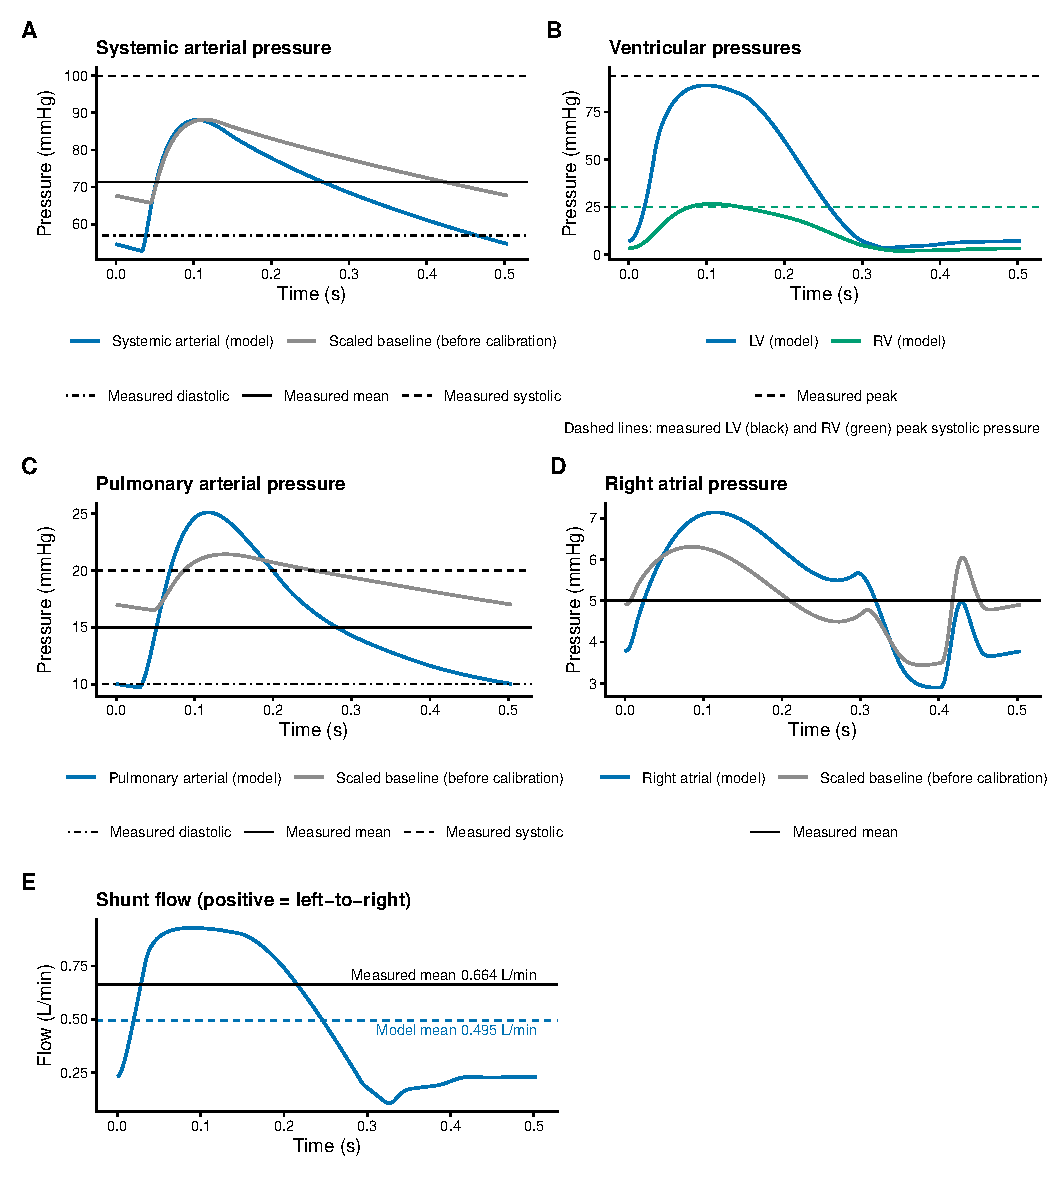
\includegraphics[width=0.95\linewidth]{M2_pre_waveforms.pdf}
\caption{Calibrated pre-closure waveforms over one cardiac cycle (blue) against the catheter measurements (black horizontal lines), with the scaled baseline before calibration (grey). (A) Systemic arterial pressure against RFA systolic, diastolic and mean pressure. (B) LV and RV pressure against the measured peak systolic pressures. (C) PA pressure. (D) RA pressure. (E) Shunt flow and its cycle mean against the Fick-derived shunt flow.}
\label{fig:pre_waves}
\end{figure}

\FloatBarrier
\subsection{Simulated pre-closure hemodynamics}
\label{sec:results_hemo}
The calibrated model gave a pulmonary flow of 3.64~L/min, a systemic flow of 3.15~L/min and a mean LA pressure of 7.85~mmHg; the shunt carried 13.6\% of pulmonary flow. The chamber volumes, which have no pre-closure measurement, were LVEDV 39.8~mL, LVESV 9.8~mL and LVEF 0.75, and RVEDV 43.3~mL, RVESV 14.9~mL and RVEF 0.65 (Table~\ref{tab:pre_targets}). No measurement constrains these volumes: the parameters that control them were below the screening threshold for every fitted target (Section~\ref{sec:results_gsa}).

\FloatBarrier
\subsection{Post-closure prediction}
\label{sec:results_post}
Table~\ref{tab:post} lists every post-closure measurement beside the prediction, with the same rows, names and symbols as Table~\ref{tab:pre_targets}. For the nine quantities fitted before closure, the RMSE of relative error was 0.191 after closure against 0.105 before.

Figure~\ref{fig:post_waves} shows the predicted waveforms against the post-closure catheter readings. The relative errors of the prediction were, for systemic arterial pressure, $+1.2\%$ for systolic RFA pressure, $-6.4\%$ for mean arterial pressure and $-23.6\%$ for diastolic RFA pressure (52.0 against 68~mmHg). The same diastolic pressure was 55~mmHg by cuff and 72~mmHg in the DAo, a 17~mmHg spread across sites; the prediction is 5.5\% below the cuff value and 27.8\% below the DAo value. For the pulmonary artery they were $+3.2\%$ for diastolic, $+14.3\%$ for mean and $+40.7\%$ for systolic pressure (23.9 against 17~mmHg, $z = +8.14$), the same overshoot as before closure; mean RA pressure was $+8.2\%$. $Q_s$ was 3.17 against 2.54~L/min ($+24.8\%$) and SVR 20.4 against 27.6~WU ($-25.9\%$). $Q_p/Q_s$ equals 1.00 in the model once the defect is closed, against 0.90 measured ($+11.2\%$). For the ventricles, LVEDV was $+13.8\%$, LVESV $-15.8\%$ and LVEF $+16.1\%$; RVEDV was 43.3 against 30.5~mL ($+42.1\%$), equal to the pre-closure model RVEDV, RVESV $+14.8\%$ and RVEF $+12.5\%$. Over the seven catheter pressures, the prediction had an RMSE of 6.9~mmHg ($R^2 = 0.96$), against 5.2~mmHg ($R^2 = 0.99$) for the same seven pressures fitted before closure (Figure~\ref{fig:parity}A).

\begin{table}[!htbp]
\centering\small
\setlength{\tabcolsep}{3pt}
\caption{Post-closure record against the prediction from the calibrated pre-closure parameters with the defect closed; nothing in this table entered calibration. Rows, names and symbols are the same as in Table~\ref{tab:pre_targets}. $\sigma$, declared uncertainty; $\varepsilon$, relative error; $z = (\text{model}-\text{measured})/\sigma$; --, not measured or not defined. The last column gives $\varepsilon$ against the alternative protocol-form record where it differs from the medical record.}
\label{tab:post}
\resizebox{\linewidth}{!}{\begin{tabular}{lrrrrrr}
\toprule
\textbf{Quantity} & $\sigma$ & \textbf{Measured} & \textbf{Predicted} & $\varepsilon$ (\%) & $z$ & $\varepsilon$, protocol form (\%) \\
\midrule
\multicolumn{7}{l}{\emph{Systemic arterial pressure}} \\
Systolic pressure, RFA (mmHg) & 8.90 & 89.00 & 90.08 & $+1.2$ & $+0.12$ & -- \\
Diastolic pressure, RFA (mmHg) & 6.80 & 68.00 & 51.95 & $-23.6$ & $-2.36$ & -- \\
Mean arterial pressure, RFA (mmHg) & 3.75 & 75.00 & 70.19 & $-6.4$ & $-1.28$ & -- \\
Systolic pressure, DAo (mmHg) & -- & 104.00 & 90.08 & $-13.4$ & -- & -- \\
Diastolic pressure, DAo (mmHg) & -- & 72.00 & 51.95 & $-27.8$ & -- & -- \\
Systolic pressure, cuff (mmHg) & -- & 87.00 & 90.08 & $+3.5$ & -- & -- \\
Diastolic pressure, cuff (mmHg) & -- & 55.00 & 51.95 & $-5.5$ & -- & -- \\
\multicolumn{7}{l}{\emph{PA and RA pressure}} \\
PA systolic pressure (mmHg) & 0.85 & 17.00 & 23.92 & $+40.7$ & $+8.14$ & -- \\
PA diastolic pressure (mmHg) & 0.45 & 9.00 & 9.29 & $+3.2$ & $+0.65$ & -- \\
Mean PA pressure (mmHg) & 0.65 & 13.00 & 14.86 & $+14.3$ & $+2.86$ & -- \\
Mean RA pressure (mmHg) & 0.25 & 5.00 & 5.41 & $+8.2$ & $+1.64$ & -- \\
\multicolumn{7}{l}{\emph{Ventricular pressure}} \\
LV systolic pressure (mmHg) & -- & -- & 90.6 & -- & -- & -- \\
RV systolic pressure (mmHg) & -- & -- & 25.3 & -- & -- & -- \\
LV--RV systolic gradient (mmHg) & -- & -- & 65.4 & -- & -- & -- \\
\multicolumn{7}{l}{\emph{Flow and resistance}} \\
Pulmonary flow $Q_p$ (L/min) & -- & -- & 3.174 & -- & -- & -- \\
Systemic flow $Q_s$ (L/min) & 0.127 & 2.54 & 3.17 & $+24.8$ & $+4.97$ & -- \\
$Q_p/Q_s$ (--) & 0.045 & 0.90 & 1.00 & $+11.2$ & $+2.23$ & -- \\
Shunt flow $Q_p - Q_s$ (L/min) & -- & -- & 0.000 & -- & -- & -- \\
SVR (WU) & 5.51 & 27.56 & 20.43 & $-25.9$ & $-1.29$ & -- \\
\multicolumn{7}{l}{\emph{Ventricular volume and function}} \\
LVEDV (mL) & 3.61 & 36.13 & 41.10 & $+13.8$ & $+1.38$ & $+28.4$ \\
LVESV (mL) & 1.38 & 13.80 & 11.62 & $-15.8$ & $-1.58$ & $-50.8$ \\
RVEDV (mL) & 3.05 & 30.50 & 43.35 & $+42.1$ & $+4.21$ & -- \\
RVESV (mL) & 1.20 & 12.00 & 13.78 & $+14.8$ & $+1.48$ & -- \\
LVEF (--) & 0.062 & 0.618 & 0.717 & $+16.1$ & $+1.61$ & $+173.3$ \\
RVEF (--) & 0.061 & 0.607 & 0.682 & $+12.5$ & $+1.25$ & -- \\
\midrule
RMSE of $\varepsilon$, nine quantities fitted before closure & & & 0.191 & & & \\
$\chi^2/N$, same nine quantities ($N=9$) & & & 12.71 & & & \\
$\chi^2/N$, all quantities with declared $\sigma$ ($N=16$) & & & 9.03 & & & \\
\bottomrule
\end{tabular}}
\end{table}

Evaluated against the protocol-form record instead, the same prediction gives $-50.8\%$ for LVESV and $+173.3\%$ for LVEF (Table~\ref{tab:post}, last column). The prediction does not change; only the reference changes. Deciding between the two records requires the source echocardiography report, which is not filed with the study data.

\begin{figure}[!htbp]
\centering
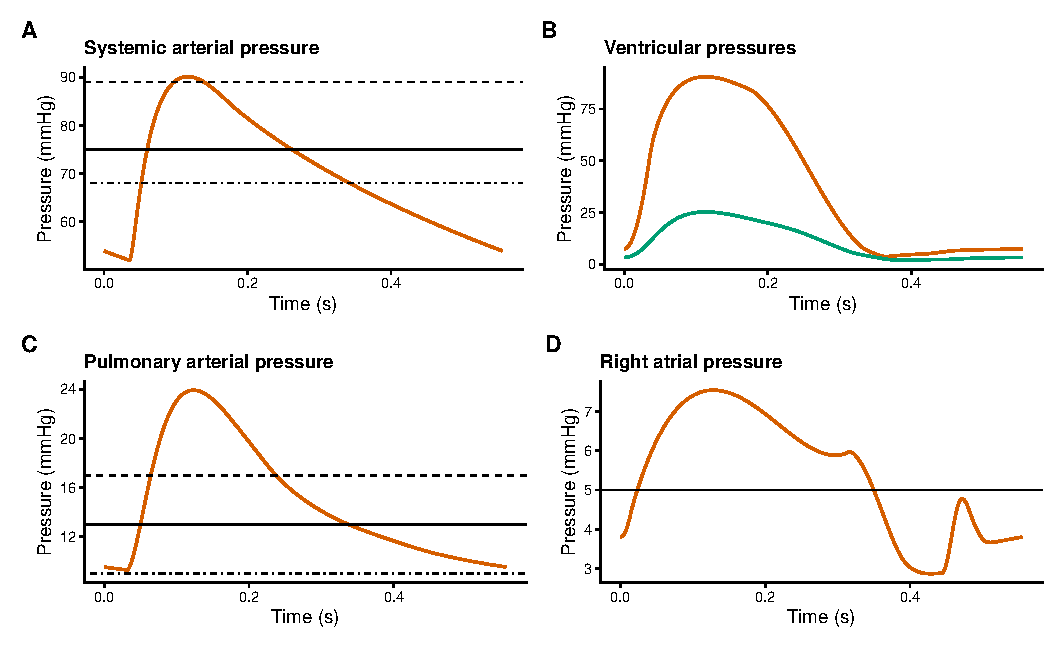
\includegraphics[width=0.95\linewidth]{M3_post_waveforms.pdf}
\caption{Predicted post-closure waveforms over one cardiac cycle (orange) against the post-closure catheter measurements (black horizontal lines). (A) Systemic arterial pressure against RFA systolic, diastolic and mean pressure. (B) Predicted LV and RV pressure. (C) PA pressure. (D) RA pressure. No post-closure measurement was used to obtain these waveforms.}
\label{fig:post_waves}
\end{figure}

\begin{figure}[!htbp]
\centering
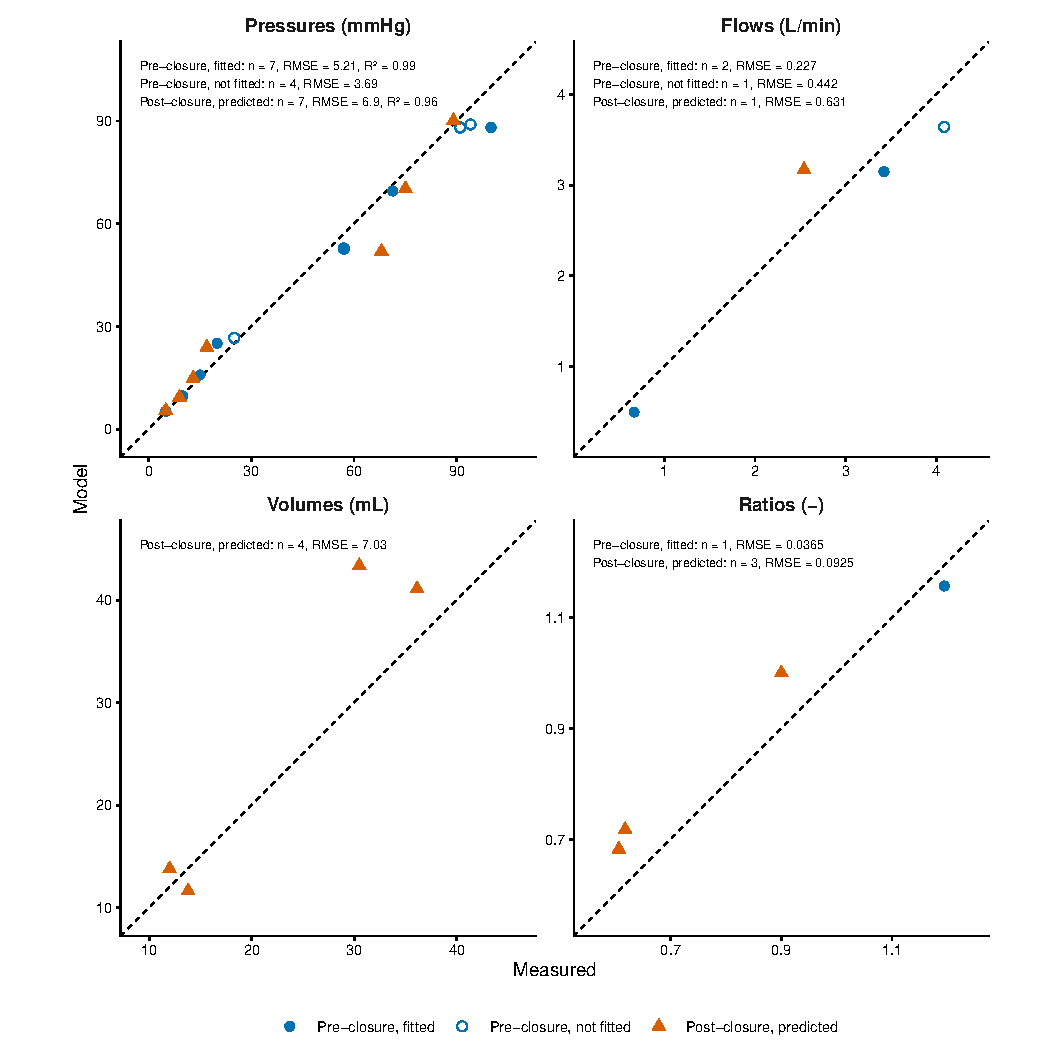
\includegraphics[width=0.9\linewidth]{M4_parity.pdf}
\caption{Model against measurement for every compared quantity. Filled circles: pre-closure targets fitted in calibration; open circles: pre-closure measurements compared but not fitted; triangles: post-closure predictions. Dashed line: identity. RMSE is in the units of each panel; $R^2$ is shown for groups of at least five points.}
\label{fig:parity}
\end{figure}

Closing the defect reduced pulmonary flow from 3.64 to 3.17~L/min ($-13\%$) and changed systemic flow from 3.15 to 3.17~L/min, so that the two became equal. Mean LA pressure changed from 7.85 to 7.92~mmHg. Because heart rate fell from 119 to 108~bpm, pulmonary venous return per beat fell only from 30.6 to 29.4~mL ($-4\%$).

\FloatBarrier
\subsection{Pressure--volume loops}
\label{sec:results_pv}
Figure~\ref{fig:pv} and Table~\ref{tab:pv} give the ventricular pressure--volume loops of the three states. Before closure, calibration raised the LV stroke volume from 21.8 to 30.0~mL and the RV stroke volume from 20.4 to 28.3~mL, and lowered the RV end-diastolic pressure from 16.5 to 9.8~mmHg. The pre-closure LV loop has no isovolumic phases: volume falls as soon as LV pressure exceeds RV pressure, because the LV ejects through the defect before the aortic valve opens. After closure, the LV loop regained its isovolumic phases, LVEDV rose from 39.8 to 41.1~mL, LVESV rose from 9.8 to 11.6~mL, LV stroke volume changed from 30.0 to 29.5~mL, and LV stroke work stayed at 0.28~J. The RV end-diastolic pressure fell from 9.8 to 4.1~mmHg, RV peak pressure from 26.7 to 25.3~mmHg, and RVEDV stayed at 43.3~mL.

\begin{figure}[!htbp]
\centering
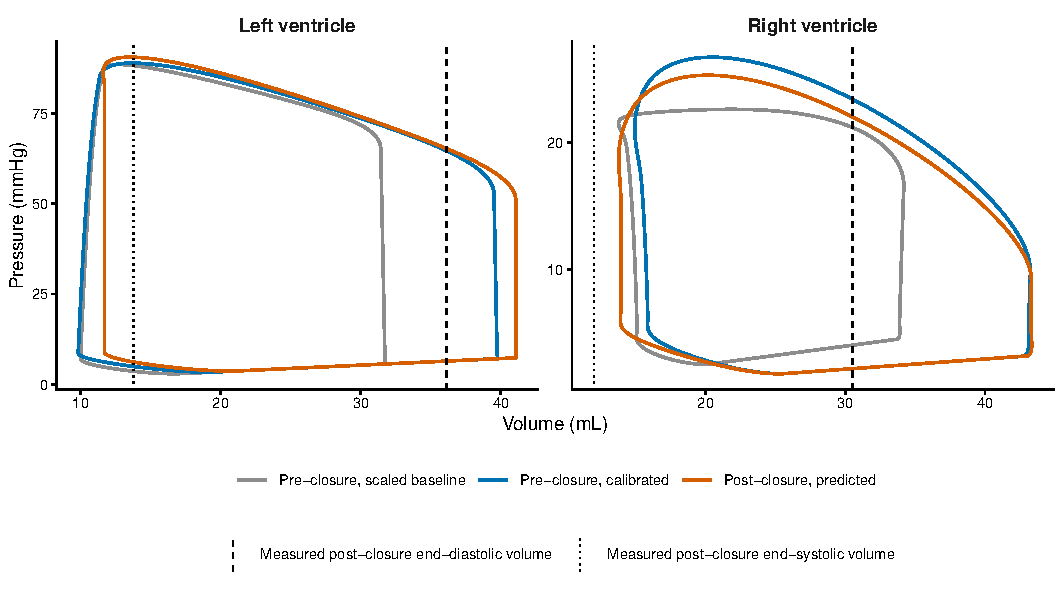
\includegraphics[width=\linewidth]{M5_pv_loops.pdf}
\caption{Left and right ventricular pressure--volume loops of the scaled baseline (grey), the calibrated pre-closure state (blue) and the post-closure prediction (orange). Vertical lines: measured post-closure end-diastolic (dashed) and end-systolic (dotted) volumes from echocardiography one day after closure.}
\label{fig:pv}
\end{figure}

\begin{table}[!htbp]
\centering\small
\setlength{\tabcolsep}{4pt}
\caption{Pressure--volume loop metrics. EDP, end-diastolic pressure; ESP, end-systolic pressure (at maximum $P/V$); SW, stroke work. Measured values exist only for post-closure volumes and ejection fractions.}
\label{tab:pv}
\begin{tabular}{llrrrr}
\toprule
& \textbf{Metric} & \textbf{Pre, baseline} & \textbf{Pre, calibrated} & \textbf{Post, predicted} & \textbf{Post, measured} \\
\midrule
\multirow{8}{*}{LV}
& EDV (mL) & 31.8 & 39.8 & 41.1 & 36.13 \\
& ESV (mL) & 10.0 & 9.8 & 11.6 & 13.80 \\
& SV (mL) & 21.8 & 30.0 & 29.5 & 22.33 \\
& EF (--) & 0.69 & 0.75 & 0.72 & 0.618 \\
& EDP (mmHg) & 6.0 & 7.4 & 7.6 & -- \\
& ESP (mmHg) & 87.4 & 86.0 & 88.6 & -- \\
& Peak pressure (mmHg) & 88.6 & 89.0 & 90.6 & -- \\
& SW (J) & 0.22 & 0.28 & 0.28 & -- \\
\midrule
\multirow{8}{*}{RV}
& EDV (mL) & 34.2 & 43.3 & 43.3 & 30.5 \\
& ESV (mL) & 13.8 & 14.9 & 13.8 & 12.0 \\
& SV (mL) & 20.4 & 28.3 & 29.6 & 18.5 \\
& EF (--) & 0.60 & 0.65 & 0.68 & 0.607 \\
& EDP (mmHg) & 16.5 & 9.8 & 4.1 & -- \\
& ESP (mmHg) & 21.7 & 24.6 & 22.9 & -- \\
& Peak pressure (mmHg) & 22.6 & 26.7 & 25.3 & -- \\
& SW (J) & 0.047 & 0.072 & 0.072 & -- \\
\bottomrule
\end{tabular}
\end{table}

\FloatBarrier
\subsection{Measurement-noise simulation}
\label{sec:results_noise}
% GENERATED by scripts/noise_section_tex.py from results/batches/noise_20260927_134251 -- do not edit by hand.
Of the 50 planned replicates, 2 had been run when this version was written: 1 was recalibrated and 1 could not start calibration because the perturbed shunt flow placed the clinically seeded $C_d$ on its lower bound. The remaining replicates use the same settings, and Tables~\ref{tab:noise_params} and \ref{tab:noise_post} and Figure~\ref{fig:noise} are regenerated from the batch output.

In the recalibrated replicate (replicate 19), $Q_s$ was 2.08~L/min against 3.42~L/min measured ($-2.7\sigma$); systolic RFA pressure was 111.3~mmHg against 100.0~mmHg measured ($+1.1\sigma$); every other perturbed target moved by less than 0.9$\sigma$. The recalibrated model fitted this perturbed record with an RMSE of relative error of 0.068 ($\chi^2/N = 1.08$), against 0.105 and 3.48 for the reference calibration to the measured record. Relative to the reference calibration, the parameters changed as follows: the systemic resistance scale from 0.5686 to 1.0922 ($+92\%$), $R_{\mathrm{SVEN}}$ from 0.1655 to 0.0817 ($-51\%$), the pulmonary resistance scale from 0.4500 to 0.6818 ($+51\%$), $C_{\mathrm{SAR}}$ from 0.5703 to 0.4177 ($-27\%$), $C_{\mathrm{PAR}}$ from 1.0170 to 1.2895 ($+27\%$), $E_{\mathrm{B,RV}}$ from 0.0799 to 0.1929 ($+141\%$) and $C_d$ from 0.3697 to 0.2140 ($-42\%$) (Table~\ref{tab:noise_params}, Figure~\ref{fig:noise}A). The post-closure prediction of this replicate differed from the reference prediction as follows: systolic pressure, RFA 90.08 to 101.10 against 89.00 measured; PA systolic pressure 23.92 to 18.94 against 17.00 measured; $Q_s$ 3.17 to 2.17 against 2.54 measured; LVEDV 41.10 to 33.32 against 36.13 measured; RVEDV 43.35 to 31.91 against 30.50 measured (Table~\ref{tab:noise_post}, Figure~\ref{fig:noise}B).

\begin{table}[!htbp]
\centering\small
\caption{Calibrated parameters across the measurement-noise replicates ($n = 1$ recalibrated of 2 run, 50 planned). Reference: the calibration to the unperturbed record (Table~\ref{tab:bounds}). SD, CV and the 2.5--97.5th percentile interval need at least two replicates; -- where not yet defined.}
\label{tab:noise_params}
\begin{tabular}{lrrrrr}
\toprule
\textbf{Parameter} & \textbf{Reference} & \textbf{Mean $\pm$ SD} & \textbf{Change (\%)} & \textbf{CV (\%)} & \textbf{95\% interval} \\
\midrule
$R_{\mathrm{sys}}$ scale & 0.5686 & 1.0922 & $+92.1$ & -- & -- \\
$R_{\mathrm{SVEN}}$ (mmHg\,s/mL) & 0.1655 & 0.0817 & $-50.7$ & -- & -- \\
$R_{\mathrm{pul}}$ scale & 0.4500 & 0.6818 & $+51.5$ & -- & -- \\
$C_{\mathrm{SAR}}$ (mL/mmHg) & 0.5703 & 0.4177 & $-26.8$ & -- & -- \\
$C_{\mathrm{PAR}}$ (mL/mmHg) & 1.0170 & 1.2895 & $+26.8$ & -- & -- \\
$E_{\mathrm{B,RV}}$ (mmHg/mL) & 0.0799 & 0.1929 & $+141.4$ & -- & -- \\
$C_d$ (--) & 0.3697 & 0.2140 & $-42.1$ & -- & -- \\
\bottomrule
\end{tabular}
\end{table}

\begin{table}[!htbp]
\centering\small
\setlength{\tabcolsep}{3pt}
\caption{Post-closure prediction across the measurement-noise replicates ($n = 1$), beside the unperturbed post-closure record and the reference prediction (Table~\ref{tab:post}). Rows, names and symbols as in Table~\ref{tab:post}; $\varepsilon$, relative error of the mean against the measurement; -- where not yet defined.}
\label{tab:noise_post}
\resizebox{\linewidth}{!}{\begin{tabular}{lrrrrr}
\toprule
\textbf{Quantity} & \textbf{Measured} & \textbf{Reference prediction} & \textbf{Mean $\pm$ SD} & $\varepsilon$ (\%) & \textbf{95\% interval} \\
\midrule
Systolic pressure, RFA (mmHg) & 89.00 & 90.08 & 101.10 & $+13.6$ & -- \\
Diastolic pressure, RFA (mmHg) & 68.00 & 51.95 & 63.74 & $-6.3$ & -- \\
Mean arterial pressure, RFA (mmHg) & 75.00 & 70.19 & 82.16 & $+9.5$ & -- \\
PA systolic pressure (mmHg) & 17.00 & 23.92 & 18.94 & $+11.4$ & -- \\
PA diastolic pressure (mmHg) & 9.00 & 9.29 & 9.15 & $+1.6$ & -- \\
Mean PA pressure (mmHg) & 13.00 & 14.86 & 13.50 & $+3.8$ & -- \\
Mean RA pressure (mmHg) & 5.00 & 5.41 & 5.65 & $+12.9$ & -- \\
Systemic flow $Q_s$ (L/min) & 2.54 & 3.17 & 2.17 & $-14.7$ & -- \\
$Q_p/Q_s$ (--) & 0.90 & 1.00 & 1.00 & $+11.1$ & -- \\
SVR (WU) & 27.56 & 20.43 & 35.29 & $+28.1$ & -- \\
LVEDV (mL) & 36.13 & 41.10 & 33.32 & $-7.8$ & -- \\
LVESV (mL) & 13.80 & 11.62 & 13.14 & $-4.8$ & -- \\
RVEDV (mL) & 30.50 & 43.35 & 31.91 & $+4.6$ & -- \\
RVESV (mL) & 12.00 & 13.78 & 11.59 & $-3.4$ & -- \\
LVEF (--) & 0.618 & 0.717 & 0.606 & $-2.0$ & -- \\
RVEF (--) & 0.607 & 0.682 & 0.637 & $+5.0$ & -- \\
\bottomrule
\end{tabular}}
\end{table}

\begin{figure}[!htbp]
\centering
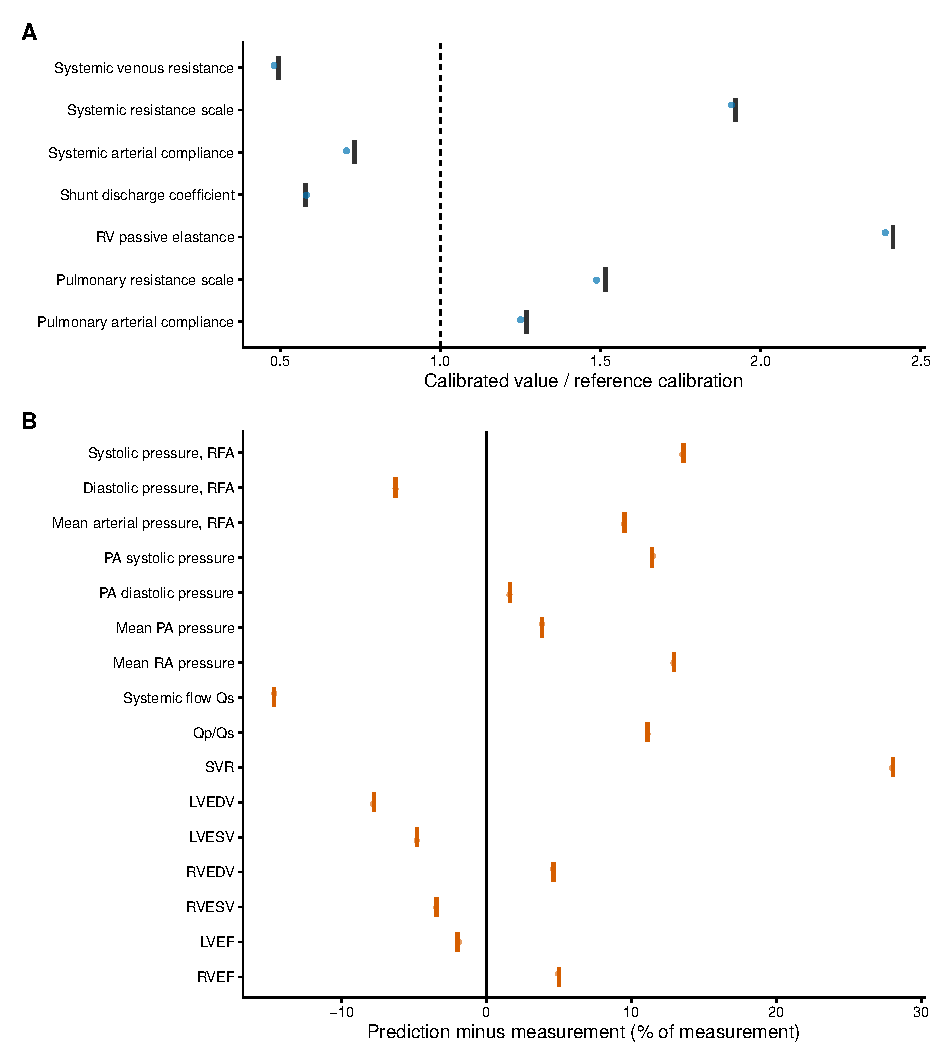
\includegraphics[width=\linewidth]{M6_noise.pdf}
\caption{Measurement-noise simulation ($n = 1$ recalibrated replicates). (A) Each calibrated parameter divided by its value in the reference calibration, one point per replicate; dashed line: reference. (B) Post-closure prediction minus measurement (\% of measurement), one point per replicate; the vertical line marks zero.}
\label{fig:noise}
\end{figure}



% =====================================================================
\FloatBarrier
\section{Discussion}
\label{sec:discussion}

\subsection{Principal findings}
This study calibrated a closed-loop lumped-parameter model to the pre-closure catheterization record of one child with a restrictive perimembranous VSD and predicted the post-closure state of the same child without refitting. Five findings follow. First, seven of fourteen candidate parameters governed the nine measured pre-closure targets, and at the scaled baseline the dominant parameter of each target was the determinant that established physiology assigns to it (Table~\ref{tab:physio_gsa}). Second, calibrating those seven reduced the RMSE of relative error over the nine fitted targets from 0.274 to 0.105, and the catheter measurements that were not fitted had relative errors between $-10.8\%$ and $+6.7\%$. Third, the simulated shunt behaved as a restrictive defect: left-to-right throughout the cycle, driven by a 62~mmHg LV--RV gradient and insensitive to pulmonary resistance. Fourth, the simulated response to closure reproduced the direction of the flow changes and of every measured pressure change that the physiology of shunt removal predicts, but not the expected left-heart unloading: LA pressure and LVEDV did not fall (Table~\ref{tab:physio_closure}). Fifth, the post-closure errors fall into three groups: an error carried over from calibration (systolic PA pressure), disagreement between measurement sites and methods (diastolic systemic pressure, $Q_s$), and chamber volumes that no pre-closure measurement constrains.

\subsection{Agreement of the sensitivity structure with established physiology}
Table~\ref{tab:physio_gsa} sets the dominant parameters found by the screen beside the determinant that clinical physiology assigns to each output. Seven of the nine comparisons agree; two agree in part.

\begin{table}[!htbp]
\centering\small
\setlength{\tabcolsep}{3pt}
\caption{Dominant parameters of the sensitivity screen at the scaled baseline (largest total-order indices, Figure~\ref{fig:gsa}) against the established physiological determinant of each output. $C_{\mathrm{SVEN}}$ was screened but is not a calibration candidate (Section~\ref{sec:gsa}).}
\label{tab:physio_gsa}
\footnotesize
\begin{tabularx}{\linewidth}{>{\raggedright\arraybackslash}p{2.2cm} >{\raggedright\arraybackslash}X >{\raggedright\arraybackslash}X >{\raggedright\arraybackslash}p{2.2cm}}
\toprule
\textbf{Output} & \textbf{Dominant parameters in the screen ($S_T$)} & \textbf{Established determinant} & \textbf{Agreement} \\
\midrule
$Q_p/Q_s$ & $C_d$ 0.51; systemic resistance 0.41; pulmonary resistance 0.01 & restrictive VSD: defect size and LV--RV gradient~\cite{Rao2024,Haas_2024} & consistent \\
Mean arterial pressure, RFA & systemic resistance 0.58 & $Q_s \times$ SVR & consistent \\
Diastolic pressure, RFA & systemic resistance 0.70 & diastolic runoff through SVR & consistent \\
Systolic pressure, RFA & systemic resistance 0.43; $C_{\mathrm{PAR}}$ 0.13; $C_{\mathrm{SAR}}$ 0.12 & mean pressure plus stroke volume over arterial compliance~\cite{FloresGeronimo2021} & partly: compliance weaker than expected \\
Mean and diastolic PA pressure & pulmonary resistance 0.30 and 0.40 & PVR, the steady component of RV afterload~\cite{Kempton2025,Gouwy2025} & consistent \\
Systolic PA pressure & $C_{\mathrm{PAR}}$ 0.39; pulmonary resistance 0.19 & PA compliance, the pulsatile component of RV afterload~\cite{Kempton2025,Gouwy2025} & consistent at the baseline; at the calibrated operating point resistance dominates (0.25) \\
Mean RA pressure & $E_{\mathrm{B,RV}}$ 0.48; $C_{\mathrm{PAR}}$ 0.14; $C_{\mathrm{SVEN}}$ 0.11 & RV filling properties and mean systemic filling pressure~\cite{Persichini2022} & consistent \\
Systemic flow $Q_s$ & systemic resistance 0.33; $C_{\mathrm{PAR}}$ 0.16; $C_{\mathrm{SVEN}}$ 0.14 & venous return: mean systemic filling pressure, RA pressure, resistance to venous return~\cite{Persichini2022} & partly: stressed blood volume not screened \\
LVESV, LVEF; RVESV, RVEF & $E_{\mathrm{A,LV}}$ 0.59, 0.63; $E_{\mathrm{A,RV}}$ 0.71, 0.76 & contractility relative to arterial load (ventricular--arterial coupling)~\cite{Vriz2021} & consistent \\
\bottomrule
\end{tabularx}
\end{table}

\paragraph{The shunt.} In a restrictive defect the orifice limits flow, and the pressure difference between the ventricles, not the ratio of pulmonary to systemic resistance, sets the shunt~\cite{Rao2024,Haas_2024}. The screen reproduces this hierarchy. $Q_p/Q_s$ depended on the discharge coefficient ($S_T = 0.51$), which scales the effective orifice area, and on systemic resistance ($S_T = 0.41$), which sets LV systolic pressure and therefore the driving gradient; pulmonary resistance had $S_T = 0.01$. The simulated LV--RV peak gradient was 62.3~mmHg against 69~mmHg measured, and RV systolic pressure was 30\% of LV systolic pressure, the pressure relation of a restrictive defect. The orifice law of Eq.~(\ref{eq:orifice}) is the same Bernoulli relation clinicians apply to the Doppler jet velocity to derive the VSD gradient and estimate RV systolic pressure~\cite{Uppu2022}, so the calibrated $C_d$ has a direct clinical counterpart. For a nonrestrictive defect the same physiology predicts the opposite hierarchy, with pulmonary resistance dominating $Q_p/Q_s$; the retained parameter set is therefore specific to the defect type and should be re-screened for each patient rather than fixed across a cohort.

\paragraph{Systemic and pulmonary pressures.} Mean and diastolic systemic pressure followed systemic resistance, as the steady pressure--flow relation requires. Systolic systemic pressure depended on resistance ($S_T = 0.43$) more than on arterial compliance ($S_T = 0.12$), whereas pulse pressure physiology gives compliance a larger role in the systolic value~\cite{FloresGeronimo2021}. The narrow sampling range of $C_{\mathrm{SAR}}$ around a value already anchored to the measured stroke volume and pulse pressure explains part of this difference. In the pulmonary circuit the screen separated the steady and pulsatile components of RV afterload exactly as clinical hemodynamics does: pulmonary resistance set the mean and diastolic PA pressure, and PA compliance set the systolic value. Kempton et al.\ showed that PVR and PA compliance computed as stroke volume over pulse pressure together describe global RV afterload~\cite{Kempton2025}, and Gouwy et al.\ showed in children with pulmonary arterial hypertension that PA compliance carries information independent of PVR~\cite{Gouwy2025}. The model's $C_{\mathrm{PAR}}$ seed uses the same stroke-volume-over-pulse-pressure definition (Table~\ref{tab:seeding}). This separation holds at the scaled baseline; at the calibrated operating point, where $C_{\mathrm{PAR}}$ was sampled over a narrower absolute range, pulmonary resistance also dominated systolic PA pressure ($S_T = 0.25$).

\paragraph{Filling pressure and systemic flow.} Mean RA pressure depended on RV passive elastance ($S_T = 0.48$) and, to a lesser extent, on systemic venous compliance, which matches the view that RA pressure reflects both RV filling properties and the mean systemic filling pressure~\cite{Persichini2022}. Systemic flow depended on systemic resistance, pulmonary arterial compliance and systemic venous compliance. In Guyton's framework, cardiac output ($Q_s$) at steady state equals venous return and is set by the mean systemic filling pressure, the RA pressure and the resistance to venous return~\cite{Persichini2022}; the stressed blood volume is the main determinant of the filling pressure. $C_{\mathrm{SVEN}}$, which is not calibrated directly but follows $R_{\mathrm{SVEN}}$ (Eq.~\ref{eq:rc}), exceeded the retention threshold for five fitted targets (Section~\ref{sec:results_gsa}), so its influence on RA pressure, PA pressure and $Q_s$ is carried by the calibrated parameters instead. In this model the stressed volume is fixed by the blood-volume constraint of Eq.~(\ref{eq:sven}) and was not among the screened inputs. The screen therefore assigns to arterial resistance part of the control over systemic flow that physiology assigns to venous capacitance and blood volume; this is a property of the chosen input set, not a finding about P1.

\paragraph{Chamber function.} Active elastance controlled end-systolic volume and ejection fraction of both ventricles ($S_T$ 0.59--0.76) and had $S_T < 0.10$ for every measured pressure and flow. This is the separation described by ventricular--arterial coupling: ejection fraction and end-systolic volume reflect contractility relative to arterial load, whereas mean pressures and flows are set mainly by the vascular load and venous return~\cite{Vriz2021,Persichini2022}. The consequence for this study is direct: the pre-closure catheterization contains no quantity that informs contractility, so the chamber parameters were not calibrated, and the post-closure chamber volumes are unconstrained predictions. Lechuga et al.\ found the same split in pulmonary hypertension, where sensitivity screening retained the resistances and elastances that governed measured pressure and flow~\cite{Lechuga2026}, and guidelines for mechanistic cardiovascular modeling recommend exactly this restriction of calibration to the parameters the data inform~\cite{Colebank2024Guidelines,Colunga2023}.

\subsection{Agreement of the simulated pre-closure hemodynamics with the physiology of a restrictive VSD}
The shunt stayed left-to-right throughout the cardiac cycle, with a systolic peak of 0.93~L/min and a diastolic minimum of 0.11~L/min (Figure~\ref{fig:pre_waves}E), because LV pressure exceeded RV pressure at every instant. Of the 4.2~mL shunted per beat, 6\% crossed during isovolumic contraction, 37\% during ejection, 40\% after aortic valve closure while the LV was relaxing, and 17\% during diastolic filling. The LV therefore had no true isovolumic phases before closure (Figure~\ref{fig:pv}), which is the expected mechanics of a ventricle with a second, low-pressure outlet. The split of shunt volume between systole and relaxation depends on the ventricular relaxation duration, which was taken from the adult reference and not calibrated; Doppler recording of the VSD jet over the cycle would test it directly.

The calibrated LVEF of 0.75 before closure is high, and it fell to 0.72 after closure. An LV that ejects part of its stroke volume into the low-pressure RV works against a lower effective afterload, and the loss of that outlet and of the shunt preload after closure is the mechanism proposed for the early fall in LV systolic function after VSD repair~\cite{Safa2023}. The model reproduces the direction of this change.

One pre-closure result does not agree with VSD physiology. A left-to-right VSD loads the left atrium and LV, because the shunted blood returns through the pulmonary veins~\cite{Safa2023,Rao2024}; in a perimembranous restrictive defect the RV is not the volume-loaded chamber. The calibrated model had a larger RV than LV (RVEDV 43.3~mL against LVEDV 39.8~mL), and the measured post-closure volumes show the opposite relation (RVEDV 30.5~mL against LVEDV 36.1~mL). The RV passive elastance, the only chamber parameter calibrated, reached its lower bound: the fit made the RV more compliant to hold mean RA pressure at 5~mmHg, and a compliant RV fills to a large volume. The RV volume is therefore a by-product of fitting RA pressure without a volume measurement, not a representation of the RV of P1.

\subsection{Agreement of the predicted closure response with clinical knowledge}
Table~\ref{tab:physio_closure} compares the simulated change at closure with the change that the physiology of shunt removal predicts and with the change that was measured.

\begin{table}[!htbp]
\centering\small
\setlength{\tabcolsep}{3pt}
\caption{Response to closure: change expected from the physiology of removing a left-to-right shunt, simulated change (calibrated pre-closure $\rightarrow$ predicted post-closure) and measured change. Model flows are cycle means of the continuous flow states.}
\label{tab:physio_closure}
\resizebox{\linewidth}{!}{%
\begin{tabular}{lllll}
\toprule
\textbf{Quantity} & \textbf{Expected after closure} & \textbf{Model, pre $\rightarrow$ post} & \textbf{Measured, pre $\rightarrow$ post} & \textbf{Agreement of the model} \\
\midrule
Pulmonary flow $Q_p$ (L/min) & falls to systemic flow & 3.64 $\rightarrow$ 3.17 ($-13\%$) & 4.09 $\rightarrow$ -- & consistent \\
$Q_p/Q_s$ (--) & 1.0 & 1.157 $\rightarrow$ 1.000 & 1.194 $\rightarrow$ 0.90 & consistent \\
Systemic flow $Q_s$ (L/min) & unchanged or higher & 3.15 $\rightarrow$ 3.17 & 3.42 (Fick) $\rightarrow$ 2.54 (echo) & consistent; measurement is not \\
Mean PA pressure (mmHg) & lower, with lower $Q_p$ & 15.8 $\rightarrow$ 14.9 & 15 $\rightarrow$ 13 & consistent in direction \\
Mean arterial pressure, RFA (mmHg) & unchanged or higher & 69.6 $\rightarrow$ 70.2 & 71.3 $\rightarrow$ 75.0 & consistent \\
Mean RA pressure (mmHg) & unchanged & 5.2 $\rightarrow$ 5.4 & 5 $\rightarrow$ 5 & consistent \\
LVEF (--) & lower (loss of low-pressure outlet)~\cite{Safa2023} & 0.75 $\rightarrow$ 0.72 & -- $\rightarrow$ 0.618 & consistent in direction \\
Mean LA pressure (mmHg) & lower (less pulmonary venous return) & 7.85 $\rightarrow$ 7.92 & not measured & not consistent \\
LVEDV (mL) & lower (LV unloading)~\cite{Yuan2025,Safa2023} & 39.8 $\rightarrow$ 41.1 & -- $\rightarrow$ 36.1 & not consistent \\
RVEDV (mL) & RV not volume-loaded before or after & 43.3 $\rightarrow$ 43.3 & -- $\rightarrow$ 30.5 & not consistent \\
SVR (WU) & unchanged in the model by construction & 20.4 $\rightarrow$ 20.4 & 19.4 $\rightarrow$ 27.6 & -- \\
\bottomrule
\end{tabular}}
\end{table}

\paragraph{Where the simulation agrees.} Closing the orifice removed the shunt, pulmonary flow fell by 13\% to equal systemic flow, $Q_p/Q_s$ became 1.00, and mean PA pressure fell by 1.0~mmHg; the measured mean PA pressure fell by 2~mmHg. Mean arterial pressure rose slightly in both the model ($+0.6$~mmHg) and the measurement ($+3.7$~mmHg), RA pressure stayed at about 5~mmHg in both, and LVEF fell. For a shunt of this size ($Q_p/Q_s = 1.19$, 16\% of pulmonary flow), the physiology predicts small hemodynamic changes at closure, and the simulated and measured pressure changes are both small.

\paragraph{Where the simulation does not agree.} Closure of a left-to-right shunt removes part of the pulmonary venous return to the left heart, and LV dimensions in children normalize after transcatheter VSD closure, most of the change occurring in the first month~\cite{Yuan2025}. The model predicted no left-heart unloading: mean LA pressure stayed at 7.9~mmHg and LVEDV rose from 39.8 to 41.1~mL. The cause is visible in the flows. Pulmonary venous return per minute fell by 13\%, but heart rate fell at the same time from 119 to 108~bpm, so pulmonary venous return per beat fell only from 30.6 to 29.4~mL ($-4\%$) while diastole lengthened. With chamber properties held at their pre-closure values, the LV filled to the same or a slightly larger volume. The LV of P1 was 5~mL smaller than predicted one day after closure. Two mechanisms that the model excludes by design can explain the difference: early adaptation of the LV to the acute loss of preload~\cite{Safa2023}, and changes in loading conditions during and after the procedure.

\paragraph{Where the measurement does not agree with physiology.} Two measured changes run against the expected physiology rather than against the model. Systemic flow fell from 3.42 to 2.54~L/min ($-26\%$) and $Q_p/Q_s$ fell below 1.0 after complete closure. Closure does not reduce systemic output, and after complete closure $Q_p/Q_s < 1$ is not possible without a right-to-left pathway, which the procedure did not create. The pre-closure values come from the Fick method and the post-closure values from echocardiography. In pediatric catheterization, Fick output computed with an assumed oxygen consumption has a mean bias of $+27.5\%$ against thermodilution or MRI~\cite{Ralston2023}, and Fick and MRI flows showed poor concordance in children after heart transplantation~\cite{Schramm2023}. A change of the measurement method between the two states is therefore a sufficient explanation for the measured fall in systemic flow and for the rise in derived SVR (19.4 to 27.6~WU), without a change in the circulation of P1. The model, which keeps SVR constant, cannot and should not reproduce that change.

\subsection{Sources of the largest pre-closure errors}
Systolic PA pressure is the dominant error in both states ($z = +5.10$ before and $+8.14$ after closure). The pulmonary resistance scale reached its lower bound and $C_{\mathrm{PAR}}$ stayed near its scaled value, so the model could not narrow the PA pulse pressure from 15.4~mmHg to the measured 10~mmHg while keeping the errors in mean PA pressure and $Q_p/Q_s$ small. A single pulmonary arterial compartment has one compliance for the whole arterial tree, and a narrow pulse pressure with a normal mean is the pattern such a compartment reproduces worst~\cite{Colunga2023,Kempton2025}. A proximal and distal pulmonary arterial compartment is the direct structural remedy.

Systolic RFA pressure was 11.9\% above the model, while the DAo systolic pressure recorded in the same procedure was 3.2\% above it. The model's arterial compartment is proximal, and pulse pressure rises from central to peripheral arteries~\cite{FloresGeronimo2021}; before closure the RFA reading exceeded the DAo reading by 9~mmHg, which is of that kind. After closure the order reversed (DAo 104~mmHg, RFA 89~mmHg), so the between-site difference in this record is not consistent across the two states and cannot be attributed to amplification alone. Shunt flow was the third error ($-25.3\%$). It is the difference of two Fick flows, each carrying the assumed-oxygen-consumption error described above~\cite{Ralston2023}; with the declared uncertainties ($\sigma = 0.50$~L/min on $Q_s$, 5\% on $Q_p/Q_s$) the shunt flow has a relative uncertainty of 34\%, so the 25\% error is within one standard deviation.

\subsection{Comparison with related work}
Bozkurt et al.\ optimized 23 parameters of a lumped model for three children with dilated cardiomyopathy and matched pressures, volumes and cardiac output within 10\%~\cite{Bozkurt2022}; every compared quantity in that study was also fitted. Owashi et al.\ estimated LV pressure in twelve patients with aortic stenosis with total relative errors of 11.9\% from invasive data and 12.3\% when only systolic and diastolic arterial pressure were available~\cite{Owashi2020}. Lechuga et al.\ reported $R^2$ between 0.78 and 0.89 for pulmonary pressure waveforms across four phenotypes of pulmonary hypertension~\cite{Lechuga2026}. The pre-closure fit here is of the same order (RMSE of relative error 0.105 over nine targets, pressure RMSE 5.2~mmHg), with fewer measurements and a pediatric shunt lesion. The difference is the post-closure test: those pressures were never fitted, and they had an RMSE of 6.9~mmHg. Harrod et al.\ used lumped-parameter modeling to predict secondary pulmonary hypertension arising from left ventricular diastolic dysfunction~\cite{Harrod2021}, and Kachabi et al.\ inferred pulmonary vascular parameters with quantified uncertainty before and after disease onset~\cite{Kachabi2025}; neither addressed a structural intervention in a child. Colebank et al.\ simulated VSD of three sizes over the first two years of life without calibration to individual patients~\cite{Colebank2026}, and Ferrero et al.\ used a 0D model to interpret catheterization data in intracardiac shunts without predicting a post-intervention state~\cite{Ferrero2026Shunts}. A dedicated post-closure calibration is the natural upper bound on what a forward prediction can achieve, and the gap between that bound and the forward prediction measures how much post-closure information the pre-closure record lacks.

\subsection{Measurement uncertainty}
% GENERATED -- do not edit by hand.
The completed replicate shows how strongly the calibrated parameters depend on the measured systemic flow. Its perturbed $Q_s$ was 2.08~L/min, 39\% below the measured value; a deviation of this order is comparable to the error of pediatric Fick output computed with an assumed oxygen consumption, which has a mean bias of $+27.5\%$ and a standard deviation of 30\% against thermodilution or MRI~\cite{Ralston2023}. Recalibrating to this record fitted it as closely as the reference calibration fitted the measured record (RMSE 0.068 against 0.105), but with the systemic resistance scale changed by $+92\%$ and $E_{\mathrm{B,RV}}$ by $+141\%$. Records that differ only within the declared measurement uncertainty are therefore fitted equally well by markedly different parameter sets. This agrees with the conditioning of the sensitivity matrix of the seven-parameter set (Supplementary Section~S2) and supports calibrating such models with quantified parameter uncertainty when the clinical data are limited~\cite{Kachabi2025,Colunga2023}. The same replicate predicted RVEDV at 31.9~mL and LVEDV at 33.3~mL against 30.5 and 36.1~mL measured, where the reference calibration predicted 43.3 and 41.1~mL. The post-closure volume errors of the reference prediction are therefore of the size that pre-closure measurement uncertainty alone can produce, and a volume prediction from this record should be reported with its uncertainty, as recommended for mechanistic cardiovascular models~\cite{Colebank2024Guidelines}. The 20-replicate ensemble quantifies how often such shifts occur.


% \subsection{Comparison with a healthy child of the same size}
% TODO (supervisor comment S20): add once the healthy-reference simulation has been run.

\subsection{Clinical relevance}
The calibrated model gives quantities that the catheterization record does not contain: the shunt flow over the cycle and its split between systole and relaxation, LA pressure, and the pressure--volume loops of both ventricles. Its sensitivity structure matches the physiology clinicians use to reason about a restrictive VSD, so its parameters have a clinical reading: $C_d$ corresponds to the effective defect size behind the Doppler gradient, systemic resistance to LV afterload, and PA compliance to the pulsatile RV load. After closure, the model predicts the direction of every measured catheter pressure change from pre-closure data alone, with relative errors of $+1.2\%$ for systolic and $-6.4\%$ for mean arterial pressure and $+8.2\%$ for RA pressure. It does not predict left-heart unloading or chamber volumes, and it should not be used for those purposes until a pre-closure volume measurement enters calibration and the chamber parameters are allowed to adapt at closure. Clinical decisions on closure rest on defect size, shunt magnitude and symptoms~\cite{Rao2024}; a calibrated model adds a prediction of the post-closure state for the individual child, which is the step towards the cardiovascular digital twins described in recent work~\cite{Niederer2021,Katsoulakis2024}.

\subsection{Limitations}
\begin{itemize}[leftmargin=1.5em]
\item One patient was studied; no claim of population-level performance is made.
\item Two of the seven calibrated parameters rest on their lower bounds, and systolic PA pressure remains $5.1\sigma$ above its measurement after calibration.
\item No chamber volume was measured before closure, so the chamber parameters were not calibrated; the RV volume is a by-product of fitting RA pressure, and the post-closure volumes are unconstrained predictions.
\item Chamber parameters are held fixed at closure, so the model cannot represent acute LV adaptation to the loss of shunt preload.
\item Ventricular activation and relaxation durations come from the adult reference and were not calibrated; the phase split of shunt flow depends on them.
\item The post-closure prediction describes the acute state, with the chamber properties of the pre-closure state. It does not represent the changes over the following weeks, when LV dimensions normalize~\cite{Yuan2025}. The study protocol schedules further measurements one day after closure and at the first outpatient follow-up; calibrating time-dependent chamber parameters to these measurements is the next step.
\item The post-closure pressures and volumes were measured one day apart and are treated as one state; pre- and post-closure systemic flow come from different methods (Fick and echocardiography).
\item Two records disagree on the post-closure LV volumes, and the three post-closure measurement sites disagree on diastolic systemic pressure by 17~mmHg.
\item The sensitivity screen used 128 training simulations truncated at 10 cycles, which supports ranking but not precise indices, and it did not include blood volume. Sensitivity indices depend on the operating point: the dominant parameter of systolic PA pressure changed between the baseline and the calibrated screen.
\item The venous compliances are not calibrated directly but follow their resistances through Eq.~(\ref{eq:rc}), and the atrial unstressed volumes are held at their scaled values; $C_{\mathrm{SVEN}}$ exceeded the retention threshold. The sensitivity screen sampled all inputs independently, without this coupling, so it does not describe the coupled parameter space that calibration explored.
\item No post-closure calibration was performed; the post-closure state is a forward prediction only.
\end{itemize}

% =====================================================================
\FloatBarrier
\section{Conclusion}
\label{sec:conclusion}
A closed-loop lumped-parameter model of pediatric VSD was scaled by body weight, screened by global sensitivity analysis, calibrated to one child's pre-closure catheterization, and used without refitting to predict the same child's post-closure state. Calibration reduced the RMSE of relative error over the nine fitted targets from 0.274 to 0.105, and the pre-closure measurements that were not fitted had relative errors between $-10.8\%$ and $+6.7\%$. After closure, the relative errors were $+1.2\%$ for systolic and $-6.4\%$ for mean arterial pressure, $+3.2\%$ for diastolic PA pressure and $+8.2\%$ for RA pressure; the largest were $+40.7\%$ for systolic PA pressure, an error carried over from calibration, and $+42.1\%$ for right-ventricular end-diastolic volume, which no pre-closure measurement constrains. % GENERATED -- do not edit by hand.
In the replicate recalibrated so far, perturbing the pre-closure record within its declared uncertainty changed the calibrated parameters by up to $141\%$ and the predicted RVEDV by 11.4~mL, so post-closure volume predictions from this record carry a large measurement-driven uncertainty.
 Adding a pre-closure echocardiographic volume measurement to calibration is the concrete next step this work identifies.

% =====================================================================
\FloatBarrier
\appendix
\section{Circulation equations}
\label{app:circuit}
Chamber pressures follow Eq.~(\ref{eq:elastance}); vascular pressures are $P_i = (V_i - V_{0,i})/C_i$ for $i \in \{\mathrm{SAR}, \mathrm{SC}, \mathrm{SVEN}, \mathrm{PAR}, \mathrm{PVEN}\}$, with RA, LA, systemic venous and pulmonary venous pressure bounded below at $-5$~mmHg. Valve flows follow Eq.~(\ref{eq:valve}) and the shunt Eq.~(\ref{eq:orifice}). The systemic capillary resistance is split into two halves around the capillary compliance. The vascular balances are
\begin{align}
\dot{V}_{\mathrm{SAR}} &= Q_{\mathrm{AV}} - Q_{\mathrm{SAR}}, \\
L_{\mathrm{SAR}}\dot{Q}_{\mathrm{SAR}} &= P_{\mathrm{SAR}} - P_{\mathrm{SC}} - \left(R_{\mathrm{SAR}} + \tfrac{1}{2}R_{\mathrm{SC}}\right)Q_{\mathrm{SAR}}, \\
\dot{V}_{\mathrm{SC}} &= Q_{\mathrm{SAR}} - Q_{\mathrm{SC}}, \qquad Q_{\mathrm{SC}} = \frac{P_{\mathrm{SC}} - P_{\mathrm{SVEN}}}{\tfrac{1}{2}R_{\mathrm{SC}}}, \\
\dot{V}_{\mathrm{SVEN}} &= Q_{\mathrm{SC}} - Q_{\mathrm{SVEN}}, \\
L_{\mathrm{SVEN}}\dot{Q}_{\mathrm{SVEN}} &= P_{\mathrm{SVEN}} - P_{\mathrm{RA}} - R_{\mathrm{SVEN}}Q_{\mathrm{SVEN}}, \\
\dot{V}_{\mathrm{PAR}} &= Q_{\mathrm{PV}} - Q_{\mathrm{PAR}}, \\
L_{\mathrm{PAR}}\dot{Q}_{\mathrm{PAR}} &= P_{\mathrm{PAR}} - P_{\mathrm{PC}} - R_{\mathrm{PAR}}Q_{\mathrm{PAR}}, \\
\left(C_{\mathrm{PCOX}} + C_{\mathrm{PCNO}}\right)\dot{P}_{\mathrm{PC}} &= Q_{\mathrm{PAR}} - Q_{\mathrm{PC}}, \qquad Q_{\mathrm{PC}} = \left(P_{\mathrm{PC}} - P_{\mathrm{PVEN}}\right)\left(\frac{1}{R_{\mathrm{PCOX}}} + \frac{1}{R_{\mathrm{PCNO}}}\right), \\
\dot{V}_{\mathrm{PVEN}} &= Q_{\mathrm{PC}} - Q_{\mathrm{PVEN}}, \\
L_{\mathrm{PVEN}}\dot{Q}_{\mathrm{PVEN}} &= P_{\mathrm{PVEN}} - P_{\mathrm{LA}} - R_{\mathrm{PVEN}}Q_{\mathrm{PVEN}}.
\end{align}

\section{Nominal adult reference parameters}
\label{app:nominal_parameters}
Table~\ref{tab:nominal_parameters} reports the complete nominal parameter set used before patient-specific scaling. The values were tuned from the adult sets of Valenti~\cite{Valenti2023}, Zhang et al.~\cite{zhang2019multiscale} and Bozkurt~\cite{Bozkurt2019} as described in Section~\ref{sec:model}; Supplementary Section~S6 gives the three source values of every entry.

\begin{table}[!p]
\centering\small
\caption{Nominal adult reference values used before pediatric scaling and patient-specific initialization.}
\label{tab:nominal_parameters}
\begin{tabularx}{\textwidth}{>{\raggedright\arraybackslash}p{2.7cm} >{\raggedright\arraybackslash}X >{\raggedright\arraybackslash}p{4.0cm} >{\raggedright\arraybackslash}p{2.7cm}}
\toprule
\textbf{Group} & \textbf{Parameter(s)} & \textbf{Nominal value(s)} & \textbf{Unit} \\
\midrule
Heart rate & HR & 75 & bpm \\
LV elastance & $E_{A,LV}$; $E_{B,LV}$ & 3.5; 0.08 & mmHg/mL \\
RV elastance & $E_{A,RV}$; $E_{B,RV}$ & 0.5; 0.042 & mmHg/mL \\
LA elastance & $E_{A,LA}$; $E_{B,LA}$ & 0.35; 0.20 & mmHg/mL \\
RA elastance & $E_{A,RA}$; $E_{B,RA}$ & 0.30; 0.10 & mmHg/mL \\
Chamber $V_0$ & $V_{0,RA}$; $V_{0,RV}$; $V_{0,LA}$; $V_{0,LV}$ & 3.5385; 8.4067; 2.3085; 3.5385 & mL \\
Systemic resistance & $R_{SAR}$; $R_{SC}$; $R_{SVEN}$ & 0.050; 0.80; 0.050 & mmHg\,s/mL \\
Systemic compliance & $C_{SAR}$; $C_{SC}$; $C_{SVEN}$ & 1.33; 1.000; 30.0 & mL/mmHg \\
Systemic inertance & $L_{SAR}$; $L_{SVEN}$ & $1.0\times10^{-5}$; $1.0\times10^{-5}$ & mmHg\,s$^2$/mL \\
Systemic vascular $V_0$ & $V_{0,SAR}$; $V_{0,SC}$; $V_{0,SVEN}$ & 90.9; 49.0; 450.0 & mL \\
Pulmonary resistance & $R_{PAR}$; $R_{PCOX}$; $R_{PCNO}$; $R_{PVEN}$ & 0.010; 0.0630; 1.2640; 0.020 & mmHg\,s/mL \\
Pulmonary compliance & $C_{PAR}$; $C_{PCOX}$; $C_{PCNO}$; $C_{PVEN}$ & 5.000; 0.1983; 0.0017; 13.750 & mL/mmHg \\
Pulmonary inertance & $L_{PAR}$; $L_{PVEN}$ & $1.0\times10^{-5}$; $1.0\times10^{-5}$ & mmHg\,s$^2$/mL \\
Pulmonary vascular $V_0$ & $V_{0,PAR}$; $V_{0,PCOX}$; $V_{0,PCNO}$; $V_{0,PVEN}$ & 196.0; 0; 0; 0 & mL \\
Valve resistance & $R_{valve,open}$; $R_{valve,closed}$ & $4.0\times10^{-3}$; $9.4168\times10^4$ & mmHg\,s/mL \\
Valve smoothing & $\epsilon_{valve}$; $\epsilon_{VSD}$ & 0.5; 0.1 & mmHg \\
VSD reference & $C_d$; $\rho_{blood}$; $\Delta P_{ref}$ & 0.7; 1060; 20$^{a}$ & --; kg/m$^3$; mmHg \\
Ventricular timing & $T_{c,LV}$; $T_{r,LV}$; $T_{c,RV}$; $T_{r,RV}$ & 0.265; 0.40; 0.30; 0.40 & fraction of $T_{HB}$ \\
LA timing & $t_{ac,LA}$; $T_{c,LA}$; $T_{r,LA}$ & 0.75; 0.10; 0.80 & fraction of $T_{HB}$ \\
RA timing & $t_{ac,RA}$; $T_{c,RA}$; $T_{r,RA}$ & 0.80; 0.10; 0.70 & fraction of $T_{HB}$ \\
Solver control & maximum cycles; retained cycles; cycles per batch & 80; 2; 5 & cardiac cycles \\
ODE tolerance & relative; absolute & $10^{-5}$; $10^{-6}$ & dimensionless \\
Steady-state tolerance & volume; pulmonary capillary pressure; flow & 0.1; 0.1; 0.005 & mL; mmHg; relative \\
\bottomrule
\end{tabularx}
\vspace{2pt}
{\footnotesize $^{a}$Reference gradient used to seed $C_d$ only when no gradient is measured; for P1 the seed uses half the measured LV--RV peak gradient (Table~\ref{tab:seeding}).}
\end{table}

\section*{Data availability}
The de-identified clinical record of P1 and the exported model outputs are available from the corresponding author on reasonable request, subject to the approval of the Institutional Review Board of RSAB Harapan Kita.

\section*{Code availability}
The MATLAB and R code that reproduces every result, table and figure (\texttt{run\_all.m} for the pre-closure pipeline and post-closure prediction, \texttt{run\_noise\_simulation.m} for the measurement-noise simulation) is available from the corresponding author on request.

\section*{Author contributions}
\pending{CRediT roles for each author: conceptualization, methodology, software, formal analysis, investigation, data curation, writing -- original draft, writing -- review and editing, supervision.}

\section*{Funding}
\pending{Funding source and grant number, or ``This research received no external funding.''}

\section*{Conflict of interest}
\pending{``The authors declare no conflict of interest.'' or the declared conflicts.}

\section*{Acknowledgments}
\pending{Clinical staff of RSAB Harapan Kita who acquired the data, if they are not authors.}

\clearpage
\printbibliography

\end{document}
